% \iffalse meta-comment
%
% Copyright (C) 2019-2020 by Jingxuan Yang <yanglatex2e@gmail.com>
%
% This work may be distributed and/or modified under the
% conditions of the LaTeX Project Public License, either version 1.3c
% of this license or (at your option) any later version.
% The latest version of this license is in
%      http://www.latex-project.org/lppl.txt
% and version 1.3c or later is part of all distributions of LaTeX
% version 2005/12/01 or later.
%
% This work has the LPPL1.3c maintenance status `maintained'.
%
% \fi
%
% \iffalse
%<*driver>
\ProvidesFile{hitszthesis.dtx}[2020/03/10 3.0 Dissertation Template for Harbin Institute of Technology, ShenZhen (HITSZ)]
\documentclass{ltxdoc}
\usepackage{dtx-style}

\EnableCrossrefs
\CodelineIndex
\RecordChanges

\begin{document}
  \DocInput{\jobname.dtx}
\end{document}
%</driver>
% \fi
%
% \CheckSum{0}
%
% \CharacterTable
%  {Upper-case    \A\B\C\D\E\F\G\H\I\J\K\L\M\N\O\P\Q\R\S\T\U\V\W\X\Y\Z
%   Lower-case    \a\b\c\d\e\f\g\h\i\j\k\l\m\n\o\p\q\r\s\t\u\v\w\x\y\z
%   Digits        \0\1\2\3\4\5\6\7\8\9
%   Exclamation   \!     Double quote  \"     Hash (number) \#
%   Dollar        \$     Percent       \%     Ampersand     \&
%   Acute accent  \'     Left paren    \(     Right paren   \)
%   Asterisk      \*     Plus          \+     Comma         \,
%   Minus         \-     Point         \.     Solidus       \/
%   Colon         \:     Semicolon     \;     Less than     \<
%   Equals        \=     Greater than  \>     Question mark \?
%   Commercial at \@     Left bracket  \[     Backslash     \\
%   Right bracket \]     Circumflex    \^     Underscore    \_
%   Grave accent  \`     Left brace    \{     Vertical bar  \|
%   Right brace   \}     Tilde         \~}
%
% \DoNotIndex{\newenvironment,\@bsphack,\@empty,\@esphack,\sfcode}
% \DoNotIndex{\addtocounter,\label,\let,\linewidth,\newcounter}
% \DoNotIndex{\noindent,\normalfont,\par,\parskip,\phantomsection}
% \DoNotIndex{\providecommand,\ProvidesPackage,\refstepcounter}
% \DoNotIndex{\RequirePackage,\setcounter,\setlength,\string,\strut}
% \DoNotIndex{\textbackslash,\texttt,\ttfamily,\usepackage}
% \DoNotIndex{\begin,\end,\begingroup,\endgroup,\par,\\}
% \DoNotIndex{\if,\ifx,\ifdim,\ifnum,\ifcase,\else,\or,\fi}
% \DoNotIndex{\let,\def,\xdef,\edef,\newcommand,\renewcommand}
% \DoNotIndex{\expandafter,\csname,\endcsname,\relax,\protect}
% \DoNotIndex{\Huge,\huge,\LARGE,\Large,\large,\normalsize}
% \DoNotIndex{\small,\footnotesize,\scriptsize,\tiny}
% \DoNotIndex{\centering,\raggedright,\ref}
% \DoNotIndex{\c@secnumdepth,\@startsection,\@setfontsize}
% \DoNotIndex{\ ,\@plus,\@minus,\p@,\z@,\@m,\@M,\@ne,\m@ne}
% \DoNotIndex{\@@par,\DeclareOperation,\RequirePackage,\LoadClass}
% \DoNotIndex{\AtBeginDocument,\AtEndDocument}
%
% \GetFileInfo{\jobname.dtx}
%
% \changes{v1.0}{2019/9/26}{Initial creation}
% \changes{v1.1}{2019/10/30}{Fix loading \pkg{mtpro2} bug, add \pkg{etex} package}
% \changes{v1.2}{2020/02/15}{Add two options: onerow or tworow, infoleft or infocenter, migrate settings file into cls file, initial commit on ctan}
% \changes{v2.0}{2020/02/18}{Format cls file to dtx file, regulate thesis template for HITSZ}
% \changes{v2.2}{2020/03/04}{Use \pkg{ctex} to set chinese titile and toc}
% \changes{v2.2}{2020/03/05}{Use \pkg{subeqnarray} rather than \pkg{cases} to write sub equations}
% \changes{v2.2}{2020/03/04}{Omit sections of appendix in toc}
% \changes{v2.3}{2020/03/05}{Add math font option XITS}
% \changes{v2.3}{2020/03/05}{Add boldcaption option to control the caption font}
%
% \def\indexname{索引}
% \def\glossaryname{修改记录}
% \IndexPrologue{\section{\indexname}}
% \GlossaryPrologue{\section{\glossaryname}}
%
% \definecolor{hitcolor}{RGB}{21,95,130}
% \title{\bfseries\color{hitcolor}\hitszthesis:哈尔滨工业大学(深圳)\\ 学位论文模板}
% \author{{\Large\fangsong 杨敬轩}\\[5pt]\texttt{yanglatex2e@gmail.com}\\[5pt]\texttt{yangjingxuan@stu.hit.edu.cn}}
% \date{v\fileversion\ (\filedate)}
% \maketitle\thispagestyle{empty}
%
% \vskip0.5cm
%
% \def\abstractname{\Large 摘\quad 要}
% \begin{abstract}\normalsize\vskip0.5cm
%   \hitszthesis 宏包旨在建立一个{\bfseries 规格严格、功夫到家}的哈尔滨工业大学(深圳)学位论文模板,目前包含本硕博毕业设计(论文)模板。模板的构建基于 \pkg{hitszthesis.dtx} 与 \pkg{hitszthesis.ins},在使用本模板之前,请仔细阅读\file{hitszthesis.pdf}(本文件)、\file{main.tex}(撰写示例)及\file{main.pdf}(撰写效果)。
% \end{abstract}
%
% \vskip1.5cm
% \def\abstractname{\Large 免责声明}
% \begin{abstract}
% \normalsize\noindent
% \begin{enumerate}
% \item 本模板的发布遵守 \href{http://www.latex-project.org/lppl.txt}{\LaTeX\ Project Public License 1.3c}以及其后的最新版本,使用前请认真阅读协议内
%   容。
% \item 本模板为作者根据\hitsz 教务处颁发的\UGR 与\PGR 编写而成,
% 旨在供\hitsz 毕业生撰写学位论文使用。
% \item 哈尔滨工业大学(深圳)教务处只提供毕业论文写作指南,不提供官方模板,也不会授
%   权第三方模板为官方模板,所以此模板仅为写作指南的参考实现,不保证格式审查老师
%   不提意见。任何由于使用本模板而引起的论文格式审查问题均与本模板作者无关。
% \item 任何个人或组织以本模板为基础进行修改、扩展而生成的新的专用模板,请严格遵
%   守 \href{http://www.latex-project.org/lppl.txt}{\LaTeX\ Project Public License 1.3c} 协议以及其后的最新版本。由于违犯协议而引起的任何纠纷争端均与
%   本模板作者无关。
% \end{enumerate}
% \end{abstract}
%
%
% \clearpage
% \pagestyle{fancy}
% \begin{multicols}{2}[
%   \setlength{\columnseprule}{.4pt}
%   \setlength{\columnsep}{18pt}]
%   \tableofcontents
% \end{multicols}
% \clearpage
%
% \section{模板介绍}
% \hitszthesis\ (\textbf{H}arbin \textbf{I}nstitute of \textbf{T}echnology,
% \textbf{S}hen\textbf{Z}hen \LaTeX\
% \textbf{Thesis} Template) 是为了帮助哈尔滨工业大学(深圳)毕业生撰写毕业论文而编写
% 的 \LaTeX\ 论文模板。
%
% 本文档将尽量完整的介绍模板的使用方法,如有不清楚之处可以参考示例文档或者根据
% 第~\ref{sec:howtoask} 节说明提问,有兴趣者可以联系作者参与完善此手册,非常欢迎窝工学子对本代码作出贡献。
%
% \note[注意:]{模板的作用在于减少论文写作过程中格式调整的时间。前提是遵守模板的
% 用法,否则即便用了 \textup{\hitszthesis}\ 也难以保证输出的论文符合学校规范。}
%
%
% \section{安装}
% \label{sec:installation}
%
% \hitszthesis\ 已经上传CTAN,已包含在TeXLive与MiKTeX发行版中。
% 安装方法:打开命令行,输入以下命令即可
% \begin{shell}
% $ tlmgr install hitszthesis
% \end{shell}
% 阅读本说明文档可以使用以下命令:
% \begin{shell}
% $ texdoc hitszthesis
% \end{shell}
%
% 如果要使用开发版,需自己下载,\hitszthesis\ 相关链接:
% \begin{itemize}
% \item 主页:\href{https://github.com/YangLaTeX/hitszthesis}{GitHub}
% \item 下载:\href{http://www.ctan.org/pkg/hitszthesis}{CTAN}
% \end{itemize}
%
% \subsection{模板的组成}
% 下表列出了 \hitszthesis\ 的主要文件及其功能介绍:
%
% \begin{longtable}{l|p{8cm}}
% \toprule
% {\heiti 文件(夹)} & {\heiti 功能描述}\\\midrule
% \endfirsthead
% \midrule
% {\heiti 文件(夹)} & {\heiti 功能描述}\\\midrule
% \endhead
% \endfoot
% \endlastfoot
% hitszthesis.ins & \textsc{DocStrip} 驱动文件(开发用) \\
% hitszthesis.dtx & \textsc{DocStrip} 源文件(开发用)\\\midrule
% hitszthesis.cls & 模板类文件\\
% hitszthesis.cfg & 模板配置文件\\
% hitszthesis.bst & 参考文献样式文件\\\midrule
% hitszthesis.ist & 索引样式文件\\\midrule
% reference.bib & 文档参考文献\\
% main.tex & 示例文档主文件\\
% front/ & 正文之前内容\\
% body/ & 正文内容\\
% body/ & 正文之后内容\\
% figures/ & 示例文档图片路径\\
% hitszthesis.sty & 为示例文档加载其它宏包\\\midrule
% Makefile & Makefile\\
% compile.bat & Windows 编译用脚本文件\\
% latexmkrc & latexmk 配置文件 \\
% README.md & Readme\\
% \textbf{hitszthesis.pdf} & 用户手册(本文档)\\\bottomrule
% \end{longtable}
%
% 几点说明:
% \begin{itemize}
% \item \file{hitszthesis.cls} 和 \file{hitszthesis.cfg} 可由 \file{hitszthesis.ins}
%   和 \file{hitszthesis.dtx} 生成,但为了降低同学们的使用难度,故
%   将 \file{hitszthesis.cls} 文件一起发布。
% \item 使用前请一定阅读文档:\file{hitszthesis.pdf}。
% \item 默认的生成的论文中含有丰富的格式示例,使用前请仔细阅读\file{main.pdf}。
% \end{itemize}
%
% \subsection{生成模板}
% \label{sec:generate-cls}
% \note[提示:]{若使用 \TeX 发行版自带的 \textup{\hitszthesis}\ 或 Github 上发布的版本,可忽
% 略此节,直接阅读第~\ref{sec:generate-thesis} 节。若下载 CTAN 包或者 Github 开发
% 代码,请阅读本节了解生成模板文件的步骤。}
%
% 模板解压缩后生成文件夹 \file{hitszthesis-vX.Y}\footnote{\texttt{vX.Y} 为版本
% 号。},其中包括:模板源文件(\file{hitszthesis.ins} 和 \file{hitszthesis.dtx}),示例文档
% (\file{main.tex},\file{spine.tex},\file{hitszthesis.sty}\footnote{可能用到的包
% 以及一些命令定义都放在这里,以免 \file{hitszthesis.cls} 过分臃
% 肿。},文件夹\file{figure/} 和 \file{front/} 。在使用之前需要先生成模
% 板文件和配置文件(具体命令细节请参考 \file{README.md} 和 \file{Makefile}):
%
% \begin{shell}
% $ cd hitszthesis-vX.Y
% # 生成 hitszthesis.cls 与 dtx-style.sty
% $ xetex hitszthesis.ins
%
% # 下面的命令用来生成用户手册,首先生成索引
% $ xelatex hitszthesis.dtx
% $ makeindex -s gind.ist -o hitszthesis.ind hitszthesis.idx
% $ makeindex -s gglo.ist -o hitszthesis.gls hitszthesis.glo
%
% # 最后两次编译生成说明文档 hitszthesis.pdf
% $ xelatex hitszthesis.dtx
% $ xelatex hitszthesis.dtx
% \end{shell}
%
% \subsection{生成论文}
% \label{sec:generate-thesis}
% 本节介绍几种常见的生成论文的方法。用户可根据自己的情况选择。
%
% \subsubsection{\XeLaTeX}
% \label{sec:xelatex}
% 很多用户对 \LaTeX\ 命令执行的次数不太清楚。一个基本的原则是多次运行 \LaTeX\ 命
% 令直至不再出现警告。下面给出生成示例文档的详细过程(\texttt{\#} 开头的行为注
% 释),首先来看推荐的 \texttt{xelatex} 方式:
% \begin{shell}
% # 1. 发现里面的引用关系,文件后缀 .tex 可以省略
% $ xelatex main
%
% # 2. 编译参考文件源文件,生成 bbl 文件
% $ bibtex main
%
% # 3. 下面解决引用
% $ xelatex main
% $ xelatex main   # 如果不需要生成索引此时生成完整的 pdf 文件
% $ splitindex main -- -s hitszthesis.ist  # 自动生成索引
% $ xelatex main.tex  # 此时生成完整的 pdf 文件
% \end{shell}
%
% \subsubsection{latexmk}
% \label{sec:latexmk}
% \texttt{latexmk} 命令支持全自动生成 \LaTeX\ 编写的文档,并且支持使用不同的工具
% 链来进行生成,它会自动运行多次工具直到交叉引用都被解决。下面给出了一个用
% \texttt{latexmk} 调用 \texttt{xelatex} 生成最终文档的示例:
% \begin{shell}
%   $ latexmk -xelatex main.tex         # 生成论文 main.pdf
%   $ latexmk -xelatex hitszthesis.dtx  # 生成说明文档 hitszthesis.pdf
%   $ latexmk -c               # 清理编译生成的辅助文件
% \end{shell}
%
% \subsubsection{GNU make}
% \label{sec:make}
% \note[提示:]{若要使用 \texttt{make} 编译,需自行下载模板。因为 \TeX\ 发行版中
% 的 \file{Makefile} 不在当前目录。}
% 上面的方法虽然不困难,但是每次都输入还是非常麻烦,所以 \hitszthesis\ 提供了一
% 个 \file{Makefile}。如果可以使用 GNU make 工具,
% 则使用 \texttt{make} 生成文件是最方便的办法。
%
% \begin{shell}
% $ make cls       # 生成 hitszthesis.cls
% $ make doc       # 生成说明文档 hitszthesis.pdf
% $ make thesis    # 生成示例文档 main.pdf
% $ make spine     # 生成书脊 spine.pdf
% $ make all       # 生成示例文档 main.pdf 以及书脊 spine.pdf
% $ make wordcount # 统计论文字数
% $ make clean     # 清理辅助文件
% $ make cleanall  # 删除所有 pdf 文件和所有辅助文件
% \end{shell}
%
% \hitszthesis\ 的 \file{Makefile} 默认用 \texttt{latexmk} 调用\texttt{xelatex} 编
% 译。如有需要可修
% 改 \file{Makefile} 开头的参数或通过命令行传递参数(请参看 \file{README.md}),
% 进一步还可以修改 \file{latexmkrc} 进行定制。
%
% \subsubsection{compile.bat}
% \label{sec:bat}
% \changes{v2.1}{2020/02/23}{Add \file{compile.bat}, add wordcount function, regulate writing style of \file{main.tex} to use \file{input}}
% 针对windows系统,本模板提供了 \file{compile.bat} 脚本文件,
% 可以双击直接编译,也可以在命令提示符窗口中使用脚本提供的额外功能:
% \begin{shell}
% $ compile.bat cls             # 生成 hitszthesis.cls
% $ compile.bat doc             # 生成说明文档 hitszthesis.pdf
% $ compile.bat thesis          # 生成示例文档 main.pdf
% $ compile.bat spine           # 生成书脊 spine.pdf
% $ compile.bat all             # 生成示例文档 main.pdf 以及书脊 spine.pdf
% $ compile.bat wordcount       # 统计论文字数
% $ compile.bat clean           # 删除编译所产生的辅助文件
% $ compile.bat cleanall        # 删除所有 pdf 文件和所有辅助文件
% \end{shell}
%
% \subsection{升级}
% \label{sec:updgrade}
% \hitszthesis\ 升级非常简单,可以通过 \TeX\ 发行版的包管理工具自动更新发行版,
% \begin{shell}
% # 更新 hitszthesis 宏包
% $ tlmgr update hitszthesis
% # 或者直接更新全部宏包至最新版
% $ tlmgr update --all
% \end{shell}
%
% 也可以下载最新的开发版,将 \file{hitszthesis.ins},\file{hitszthesis.dtx},拷贝至工作目录覆盖相应的文件,然后运行:
% \begin{shell}
% $ xetex hitszthesis.ins
% \end{shell}
% 生成新的类文件和配置文件即可。
%
% 也可以直接拷
% 贝 \file{hitszthesis.cls},\file{hitszthesis.cfg} 和
% \file{hitszthesis.ist},免去上面命令的执行。
%
% \section{使用说明}
% \label{sec:usage}
% 本手册假定用户已经能处理一般的 \LaTeX\ 文档,并对 \BibTeX\ 有一定了解。如果
% 从来没有接触过 \TeX\ 和 \LaTeX,建议先学习相关的基础知识。
%
% \subsection{关于提问}
% \label{sec:howtoask}
% 按照优先级推荐提问的位置如下:
%
% \begin{itemize}
% \item QQ group: 1039392552
% \item Github Issues: \href{http://github.com/YangLaTeX/hitszthesis/issues}{http://github.com/YangLaTeX/hitszthesis/issues}
% \item Email: \href{mailto:yanglatex2e@gmail.com}{yanglatex2e@gmail.com}, \href{mailto:yangjingxuan@stu.hit.edu.cn}{yangjingxuan@stu.hit.edu.cn}
% \end{itemize}
%
% \subsection{示例文件}
% \label{sec:userguide}
% 模板核心文件有三
% 个:\file{hitszthesis.cls},\file{hitszthesis.cfg} 和\file{hitszthesis.bst},但是如果
% 没有示例文档用户会发现很难下手。所以推荐新用户从模板自带的示例文档入手,里面包
% 括了论文写作用到的所有命令及其使用方法,只需要用自己的内容进行相应替换就可以。
% 对于不清楚的命令可以查阅本手册。下面的例子描述了模板中章节的组织形式,来自于示
% 例文档,具体内容可以参考模板附带的 \file{main.tex}。
%
% \lstinputlisting[style=lstStyleLaTeX]{main.tex}
%
% \subsection{论文选项}
% \label{sec:option}
%
% 论文选项在\file{main.tex}文件的开头描述,此处不赘述。
%
% \subsection{中文字体}
% \label{sec:chinese-fonts}
% 正确配置中文字体是使用模板的第一步。模板调用 \CTeX\ 宏包,只提供基于
% \pkg{xeCJK} 包,使用 \XeLaTeX\ 编译的方式。
% 关于如何使用字体命令、字号等等,属于模板格式范畴,在实现细节中讨论。
% 关于中文字体安装、配置的所有问题不在本模板讨论范围。
%
% \myentry{字体}
% \DescribeMacro{\songti}
% \DescribeMacro{\fangsong}
% \DescribeMacro{\heiti}
% \DescribeMacro{\kaishu}
% 宋体、仿宋、黑体、楷体四种基本字体命令:
%
% \begin{latex}
% {\songti 乾:元,亨,利贞}
% {\fangsong 初九,潜龙勿用}
% {\heiti 九二,见龙在田,利见大人}
% {\kaishu 九三,君子终日乾乾,夕惕若,厉,无咎}
% \end{latex}
%
% \myentry{字号}
% \DescribeMacro{\chuhao}
% \DescribeMacro{\xiaochu}
% \DescribeMacro{\yihao}
% 定义字体大小,分别为:
%
% \begin{center}
% \begin{tabular}{llllll}
% \toprule
% \cs{chuhao} & \cs{xiaochu} & \cs{yihao}  & \cs{xiaoyi}    & \cs{erhao}  & \cs{xiaoer}\\
% \cs{sanhao} & \cs{xiaosan} & \cs{sihao}   & \cs{xiaosi} & \cs{wuhao}  & \cs{xiaowu}\\
%   \cs{liuhao} & \cs{xiaoliu}   & \cs{qihao}  & \cs{bahao}\\\bottomrule
% \end{tabular}
% \end{center}
%
% 使用方法为:\cs{command}\oarg{num},其中 \cs{command} 为字号命令,\meta{num} 为行距。比
% 如 \cs{xiaosi}[1.5] 表示选择小四字体,行距 1.5 倍。
%
% \begin{latex}
% {\erhao 二号}
% {\sanhao[1.5] 三号,一点五倍行距}
% {\sihao 四号}
% {\qihao[2] 七号,两倍行距}
% \end{latex}
%
% 也可以使用 \CTeX\ 定义的 \cs{zihao}\marg{num} 来切换字号,具体用法参看其文
% 档。
%
% \subsection{前文}
% \label{sec:titlepage}
% 前文内容是正文之前,含封面、摘要、目录、符号表。
% 封面信息提供两种配置方法:一是通过统一设置命 令 \cs{hitszsetup}
% 通过\emph{key=value} 形式完成;二是每个信息利用命令独立设置, 其中命令的名字跟
% \emph{key} 相同。两种方式可以交叉使用,并按顺序执行(即后来的设置会覆
% 盖前面的)。以 \texttt{c} 开头的命令跟中文(chinese)相关,\texttt{e}
% 开头则为对应的英文(english)。
%
% \DescribeMacro{\hitszsetup}
% \cs{hitszsetup} 用法与常见 \emph{key=value} 命令相同,如下:
% \begin{latex}
% \hitszsetup{
%   key1 = value1,
%   key2 = {a value, with comma},
% }
% % 可以多次调用
% \hitszsetup{
%   key3 = value3,
%   key1 = value11, % 覆盖 value1
% }
% \end{latex}
%
% \note[注意:]{\cs{hitszsetup} 使用 \pkg{kvoptions} 机制,所以配置项之间不能有空行,否则
% 会报错。}
%
% 大多数命令的使用方法都是: \cs{command}\marg{arg},例外者将具体指出。这些命令都
% 在示例文档的 \file{front/cover.tex} 中。
%
% \subsubsection{密级}
% \label{sec:setup-secret}
% \myentry{密级}
% \DescribeMacro{statesecrets}
% \DescribeMacro{natclassifiedindex}
% \DescribeMacro{intclassifiedindex}
% 定义秘密级别和国内国际索引号。
% \begin{latex}
% \hitszsetup{
% statesecrets={公开},
% natclassifiedindex={TM301.2},
% intclassifiedindex={62-5},
% }
% \end{latex}
%
% \subsubsection{论文标题}
% \myentry{论文标题}
% \DescribeMacro{ctitle}
% \DescribeMacro{etitle}
% \DescribeMacro{ctitleone}
% \DescribeMacro{ctitletwo}
% \DescribeMacro{csubtitle}
% \DescribeMacro{esubtitle}
% 中英文标题。
% 如果有副标题,需要在封面选项中设置subtitle=true,否则不显示副标题。
% \begin{latex}
% \hitszsetup{
%   ctitlecover={封面中文题目可断行},
%   ctitle={论文中文题目},
%   etitle={Thesis English Title},
%   csubtitle={论文中文副题目(如果有)},
%   esubtitle={Thesis English Sub-Title (if necessary)},
%   ctitleone={本科生论文中文题目上部分},
%   ctitletwo={本科生论文中文题目下部分},
% }
% \end{latex}
%
% \subsubsection{作者姓名}
% \myentry{作者姓名}
% \DescribeMacro{cauthor}
% \DescribeMacro{eauthor}
% 作者姓名。
% \begin{latex}
% \hitszsetup{
%   cauthor={中文姓名},
%   eauthor={Name in Pinyin}
% }
% \end{latex}
%
% \subsubsection{申请学位名称}
% \label{sec:degree}
% \myentry{学科名称}
% \DescribeMacro{cxueke}
% \DescribeMacro{exueke}
% 按照入学的培养计划中学科自行填写,具体学科名称不是本文档范畴。
%
% \begin{latex}
% \hitszsetup{
%   cxueke={工学},
%   exueke={Engineering},
% }
% \end{latex}
%
% \subsubsection{院系名称}
% \myentry{院系名称}
% \DescribeMacro{caffil}
% \DescribeMacro{eaffil}
% 院系名称,同上,按照入学的培养计划中学科自行填写,具体院系名称不是本文档范畴。
% \begin{latex}
% \hitszsetup{
%  caffil={机电工程与自动化学院},
%  eaffil={\emultiline[t]{School of Mechanical Engineering\\ and Automation}},
% }
% \end{latex}
% \note[注意:]{个别学院英文名过长,使用以上方法自行换行。}
%
% \subsubsection{专业名称}
% \myentry{专业名称}
% \DescribeMacro{csubject}
% \DescribeMacro{esubject}
% 专业名称,同上,按照入学的培养计划中学科自行填写,具体名称不是本文档范畴。
% \begin{latex}
% \hitszsetup{
%  csubject={机械设计制造及其自动化},
%  esubject={Mechanical Design, Manufacturing and Automation},
% }
% \end{latex}
%
% \subsubsection{导师}
% \myentry{导师}
% \DescribeMacro{csupervisor}
% \DescribeMacro{esupervisor}
% 直接导师。
% \begin{latex}
% \hitszsetup{
%   csupervisor={导师~教授},
%   esupervisor={Supervisor}
% }
% \end{latex}
%
% \myentry{副导师}
% \DescribeMacro{cassosupervisor}
% \DescribeMacro{eassosupervisor}
% 副指导教师。
% \begin{latex}
% \hitszsetup{
%   cassosupervisor={副导师~副教授},
%   eassosupervisor={2nd Boss}
% }
% \end{latex}
%
% \myentry{联合导师}
% \DescribeMacro{ccosupervisor}
% \DescribeMacro{ecosupervisor}
% 硕士生联合指导教师,博士生联合导师。
% \begin{latex}
% \hitszsetup{
%   ccosupervisor={联合导师~教授},
%   ecosupervisor={3rd Boss}
% }
% \end{latex}
%
% \subsubsection{成文日期}
% \myentry{日期}
% \DescribeMacro{cdate}
% \DescribeMacro{edate}
% 默认为当前时间,也可以自己指定。
% \begin{latex}
% \hitszsetup{
%   cdate={中文日期},
%   edate={English Date},
% }
% \end{latex}
%
% \subsubsection{学生类型}
% \myentry{学生类型}
% \DescribeMacro{cstudenttype}
% \DescribeMacro{estudenttype}
% 非全日制教育申请学位者
%(同等学力人员)、(工程硕士)、(工商管理硕士)、
%(高级管理人员工商管理硕士)、(公共管理硕士)、(中职教师)、(高校教师)等,
% 具体要求按照入学的培养计划中学科自行填写,具体名称不是本文档范畴。
% \begin{latex}
% \hitszsetup{
%   cstudenttype={同等学力人员},
%   estudenttype={Master of Art},
% }
% \end{latex}
%
% \subsubsection{学号}
% \myentry{学号}
% \DescribeMacro{cstudentid}
% 学号,具体要求按照入学的培养计划中学科自行填写。
% \begin{latex}
% \hitszsetup{
%   cstudentid={9527},
% }
% \end{latex}
%
% \subsubsection{摘要}
% \myentry{摘要正文}
% \DescribeEnv{cabstract}
% \DescribeEnv{eabstract}
% \note[说明:]{摘要正文只能用环境命令的形式,不支持 \cs{hitszsetup}。}
%
% \begin{latex}
% \begin{cabstract}
%  摘要请写在这里...
% \end{cabstract}
%
% \begin{eabstract}
%  Here comes the abstract in English...
% \end{eabstract}
% \end{latex}
%
% \myentry{关键词}
% \DescribeMacro{ckeywords}
% \DescribeMacro{ekeywords}
% 关键词用英文逗号分割写入相应的命令中,模板会解析各关键词并生成符合不同论文格式
% 要求的关键词格式。
% \begin{latex}
% \hitszsetup{
%   ckeywords={关键词 1, 关键词 2},
%   ekeywords={keyword 1, keyword 2}
% }
% \end{latex}
%
% \subsubsection{符号对照表}
% \DescribeEnv{denotation}
% 主要符号表环境,单独在文件\file{front/denotation.tex}中。
% 跟据\PGR\
% 示例中要求,窝工符号表是table环境,示例文件如下,由于窝工要求博士论文图表标题是双语,所以任何对单个标题的全局格式调整都会影响到双语标题,所以这里使用\cs{vspace},具体见实现细节中的描述。
%
% \lstinputlisting[style=lstStyleLaTeX]{front/denotation.tex}
%
% \subsubsection{目录}
% 目录不需要用户干预,自动生成,具体命令已经写在\file{main.tex} 中。
%
% \subsection{正文}
%
% \subsubsection{图和表}
% \hitsz\ 博士毕业论文要求使用中英双语图题、表题,这增加了维护难度。
% 因为现有唯一的方法是在已有的图题或表题的基础上再添加一行英语图题或表题。
% 两个题之间的距离具体多少不在\PGR\ 中要求。目前的方法是用户手动调节该距离。
% 关于图题\PGR\ 和\UGR\ 只规定了居中,并没有规定居中对其。然而评审老师很多喜欢居
% 中且居中对齐。模板默认选项是居中且居中对齐,如果不喜欢居中对齐,那么需要在
% \file{main.tex} 的文档类选项中设置选项capcenterlast=false。详细方法见前文的介绍
% 。
% \begin{hitszrgu}
% 每个图均应有图题(由图序和图名组成),图题不宜有标点符号,图名在图序之后空1个
% 半角字符排写。图序按章编排,如第1章第一个插图的图号为“图1-1”。图题置于图下,硕
% 士论文只用中文,博士论文用中、英两种文字,居中书写,中文在上,要求中文用宋体5
% 号字,英文用Times New Roman 5号字。有图注或其它说明时应置于图题之上。引用图应
% 注明出处,在图题右上角加引用文献号。图中若有分图时,分图题置于分图之下或图题之
% 下,可以只用中文书写,分图号用a)、b)等表示。图中各部分说明应采用中文(引用的外
% 文图除外)或数字符号,各项文字说明置于图题之上(有分图时,置于分图题之上)。图
% 中文字用宋体、Times New Roman字体,字号尽量采用5号字(当字数较多时可用小5号字
% ,以清晰表达为原则,但在一个插图内字号要统一)。同一图内使用文字应统一。图表中
% 物理量、符号用斜体。
% \end{hitszrgu}
%
% 单双语图题的方法如下:
% \begin{latex}
% \begin{figure}[htpb]
% \centering
% 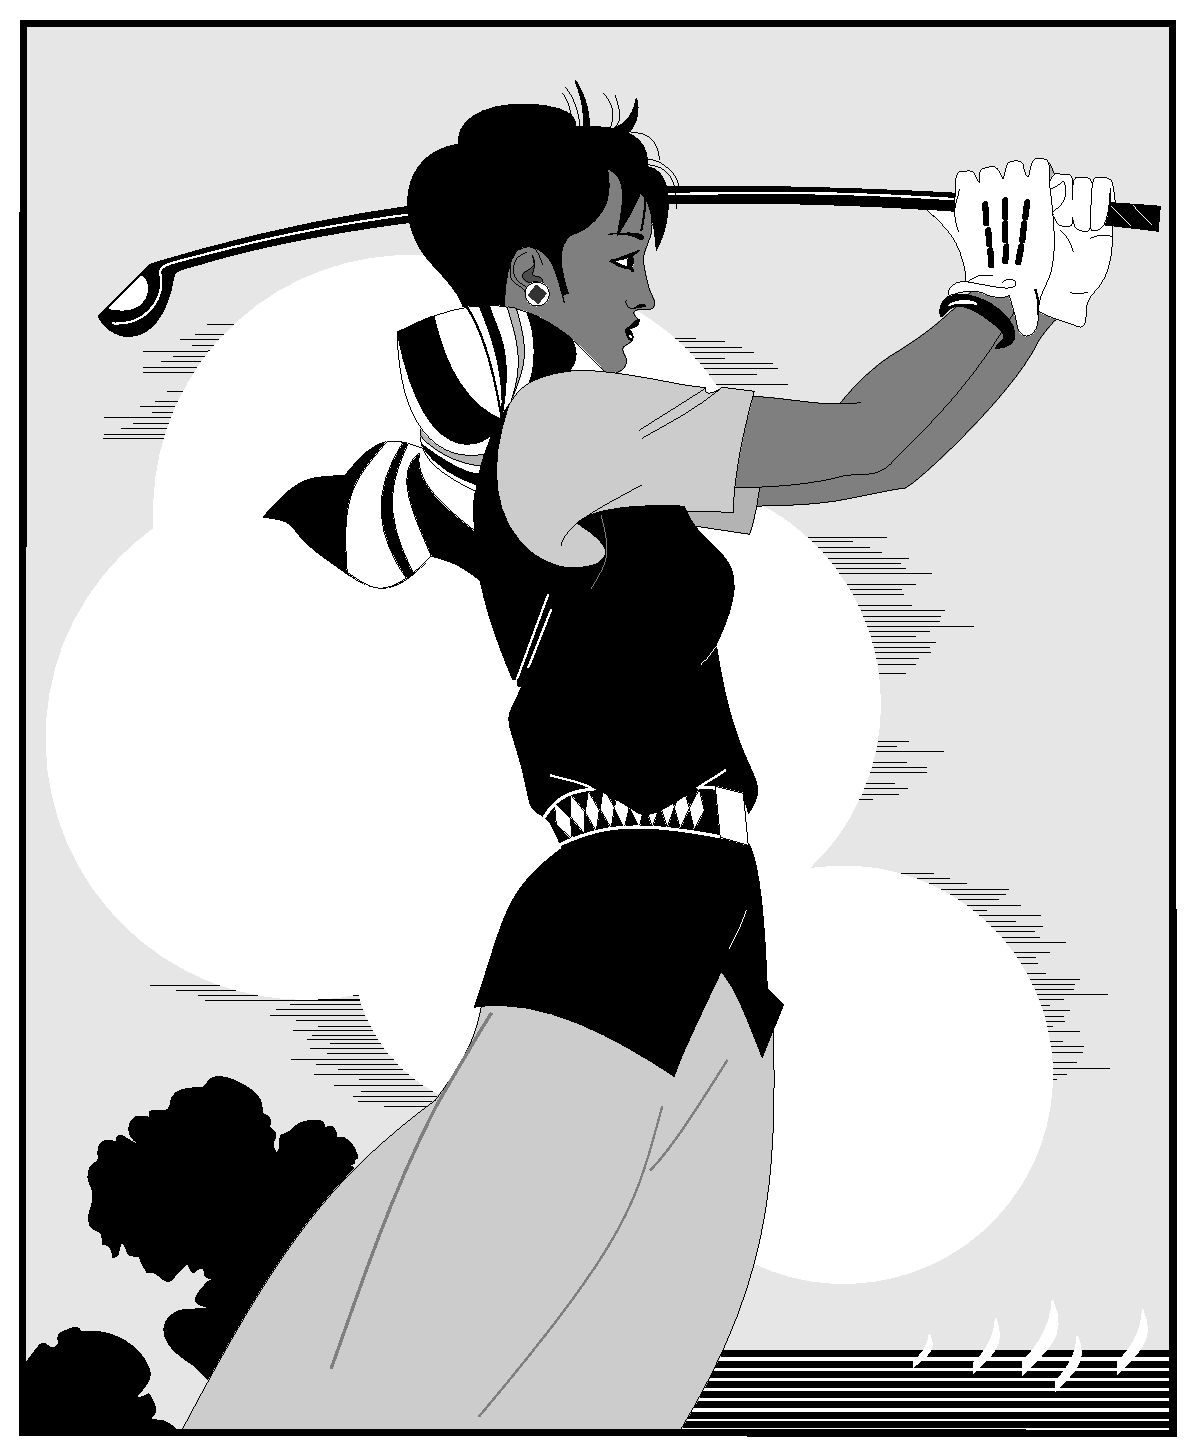
\includegraphics[width = 0.4\textwidth]{golfer}
% \bicaption[golfer1]{}{注意图中文字尽量用五号字
% }{Fig.$\!$}{The person playing golf}
% \end{figure}
% \end{latex}
%
% 单张单图题的格式如下:
% \begin{latex}
% \begin{figure}[h]
% \centering
% 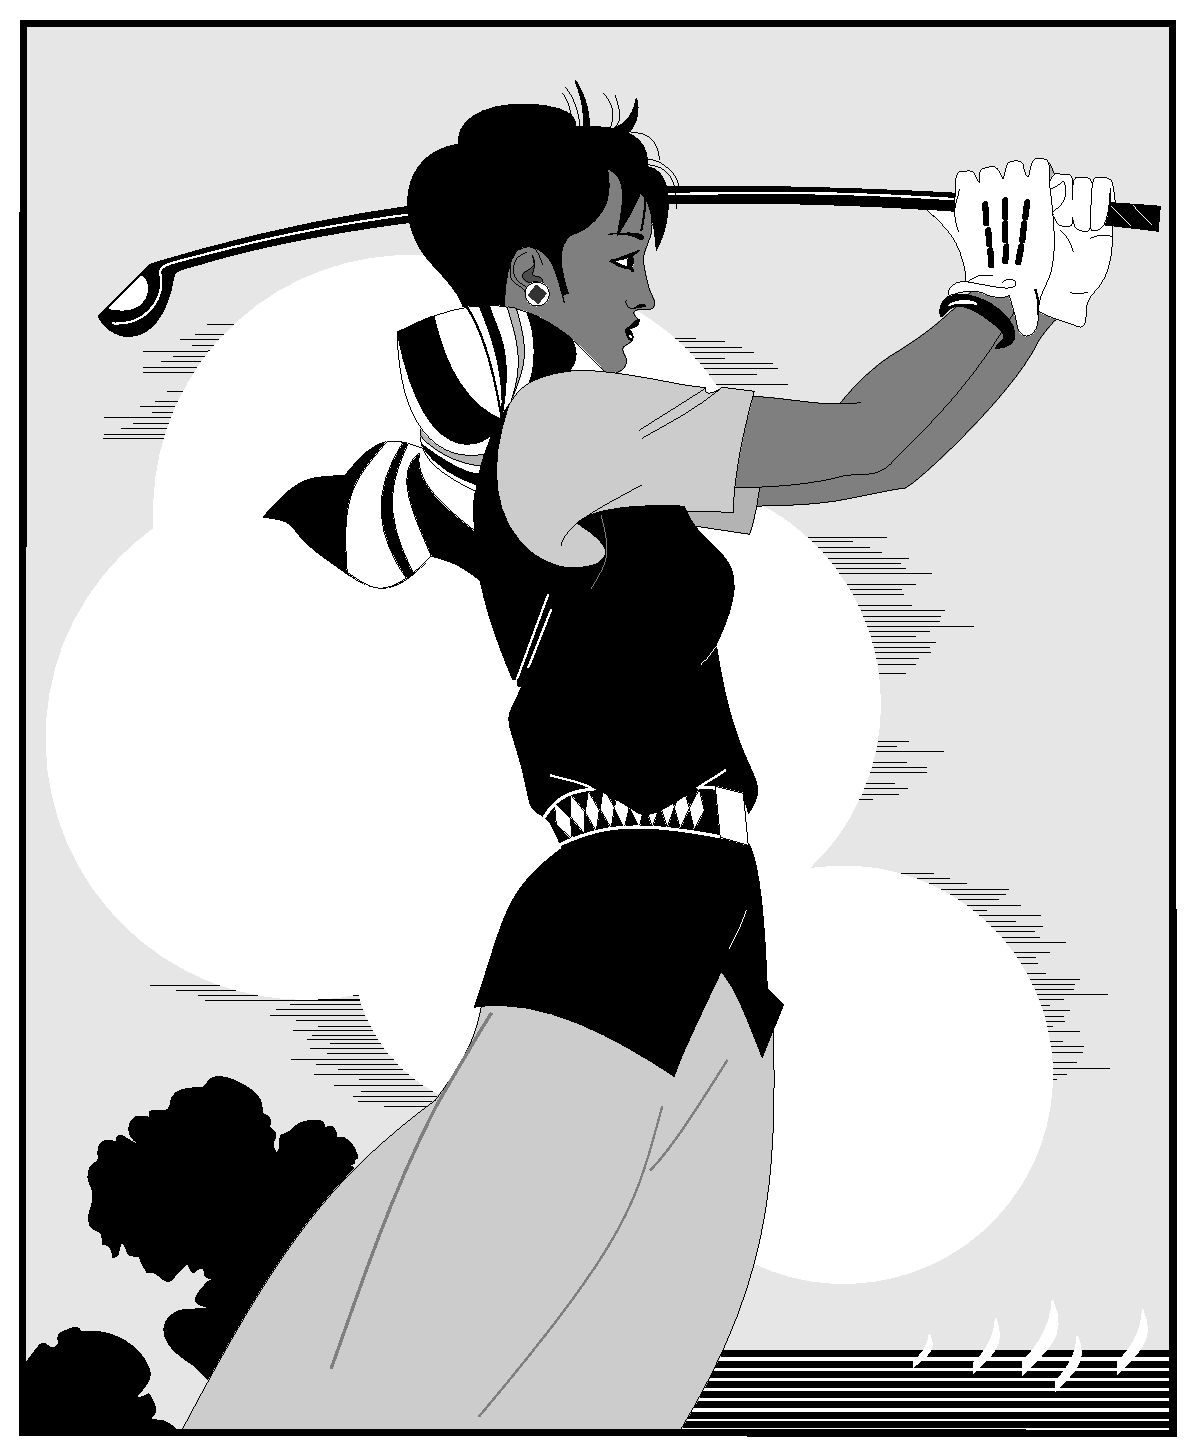
\includegraphics[width = 0.4\textwidth]{golfer}
% \caption{注意图中文字字号尽量用五号字}
% \end{figure}
% \end{latex}
%
% 并排图例:
% \begin{latex}
% \begin{figure}[htbp]
% \centering
% \begin{minipage}{0.4\textwidth}
% \centering
% 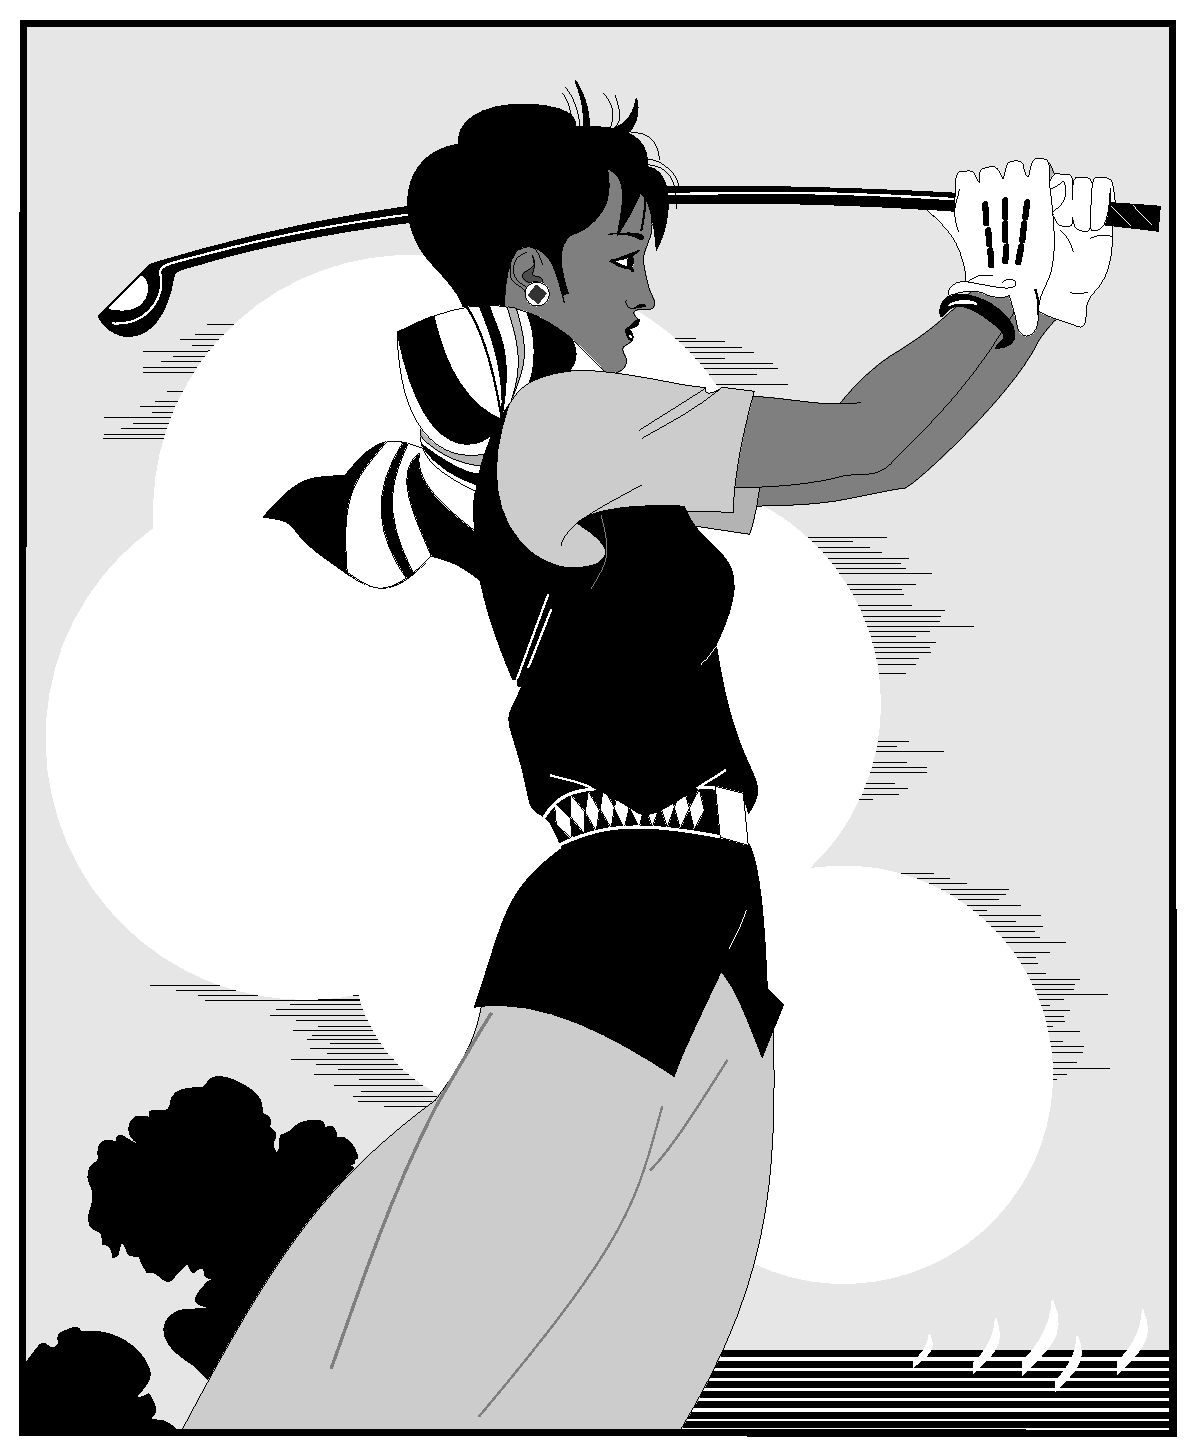
\includegraphics[width=\textwidth]{golfer}
% \bicaption[golfer2]{}{打高尔夫球的人}{Fig.$\!$}{The person playing golf}
% \end{minipage}
% \begin{minipage}{0.4\textwidth}
% \centering
% 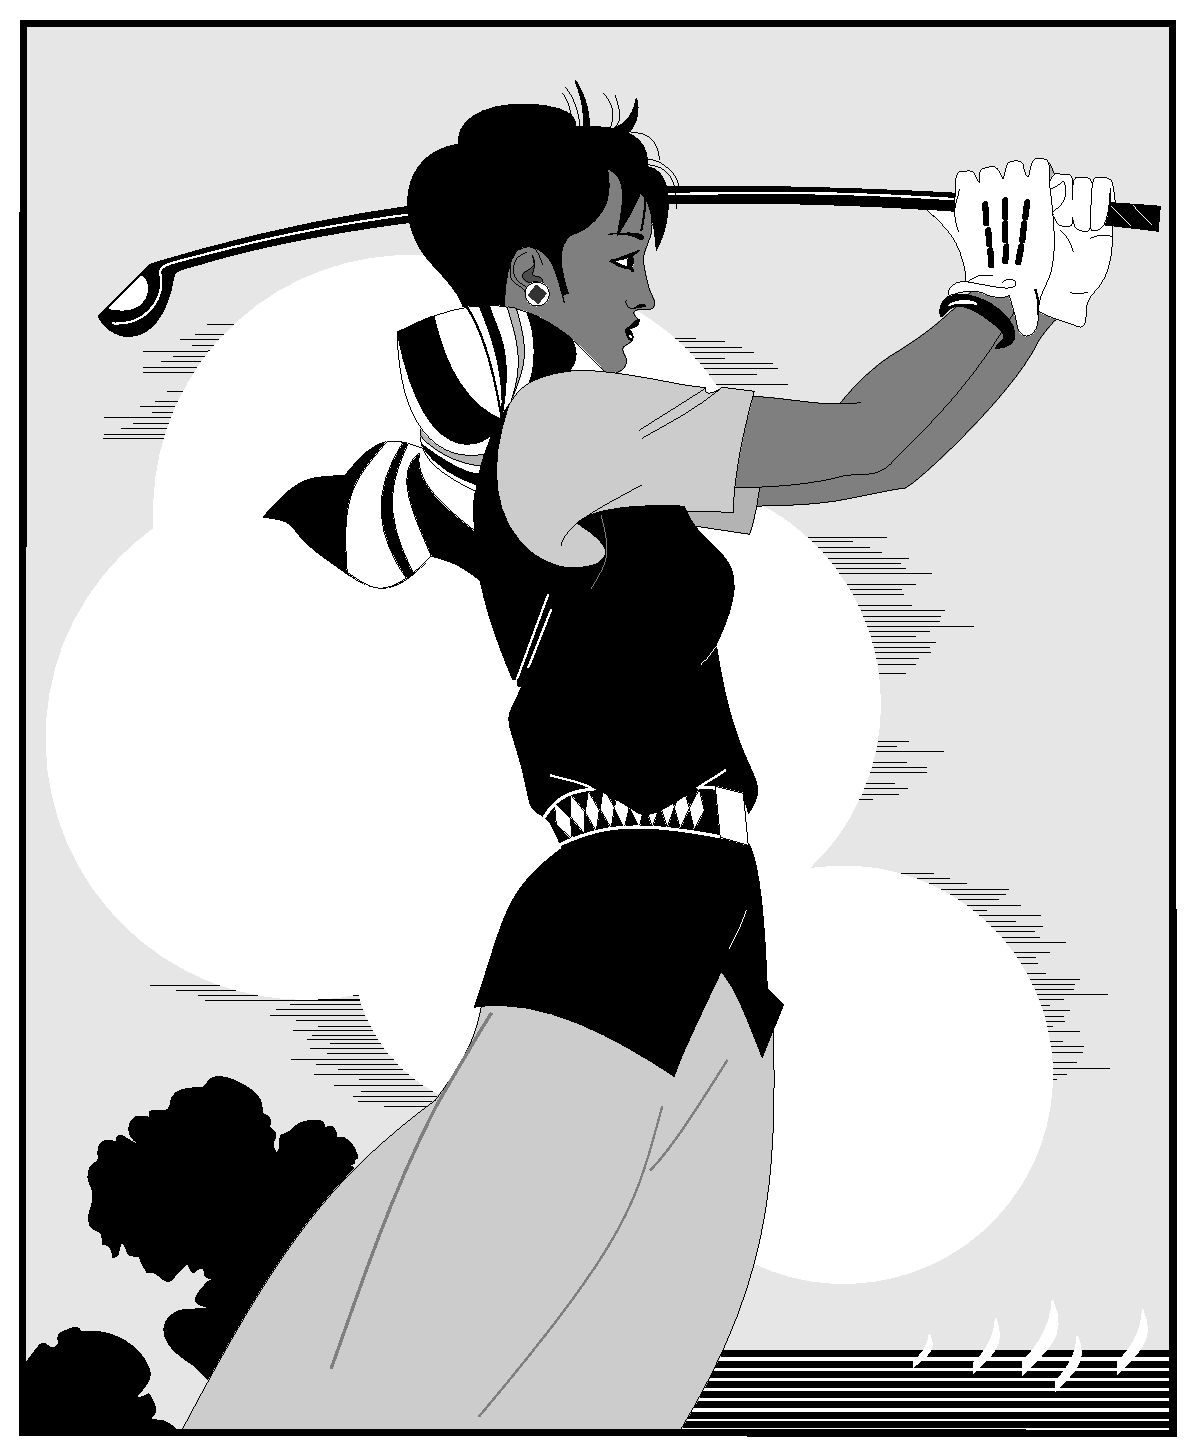
\includegraphics[width=\textwidth]{golfer}
% \bicaption[golfer3]{}{打高尔夫球的人}{Fig.$\!$}{The person playing golf}
% \end{minipage}
% \end{figure}
% \end{latex}
%
% 子图图例:
% \begin{latex}
% \begin{figure}[htbp]
% \centering
% \subfigure{\label{golfer41}}\addtocounter{subfigure}{-2}
% \subfigure[The person playing golf]{\subfigure[打高尔夫球的人~1]{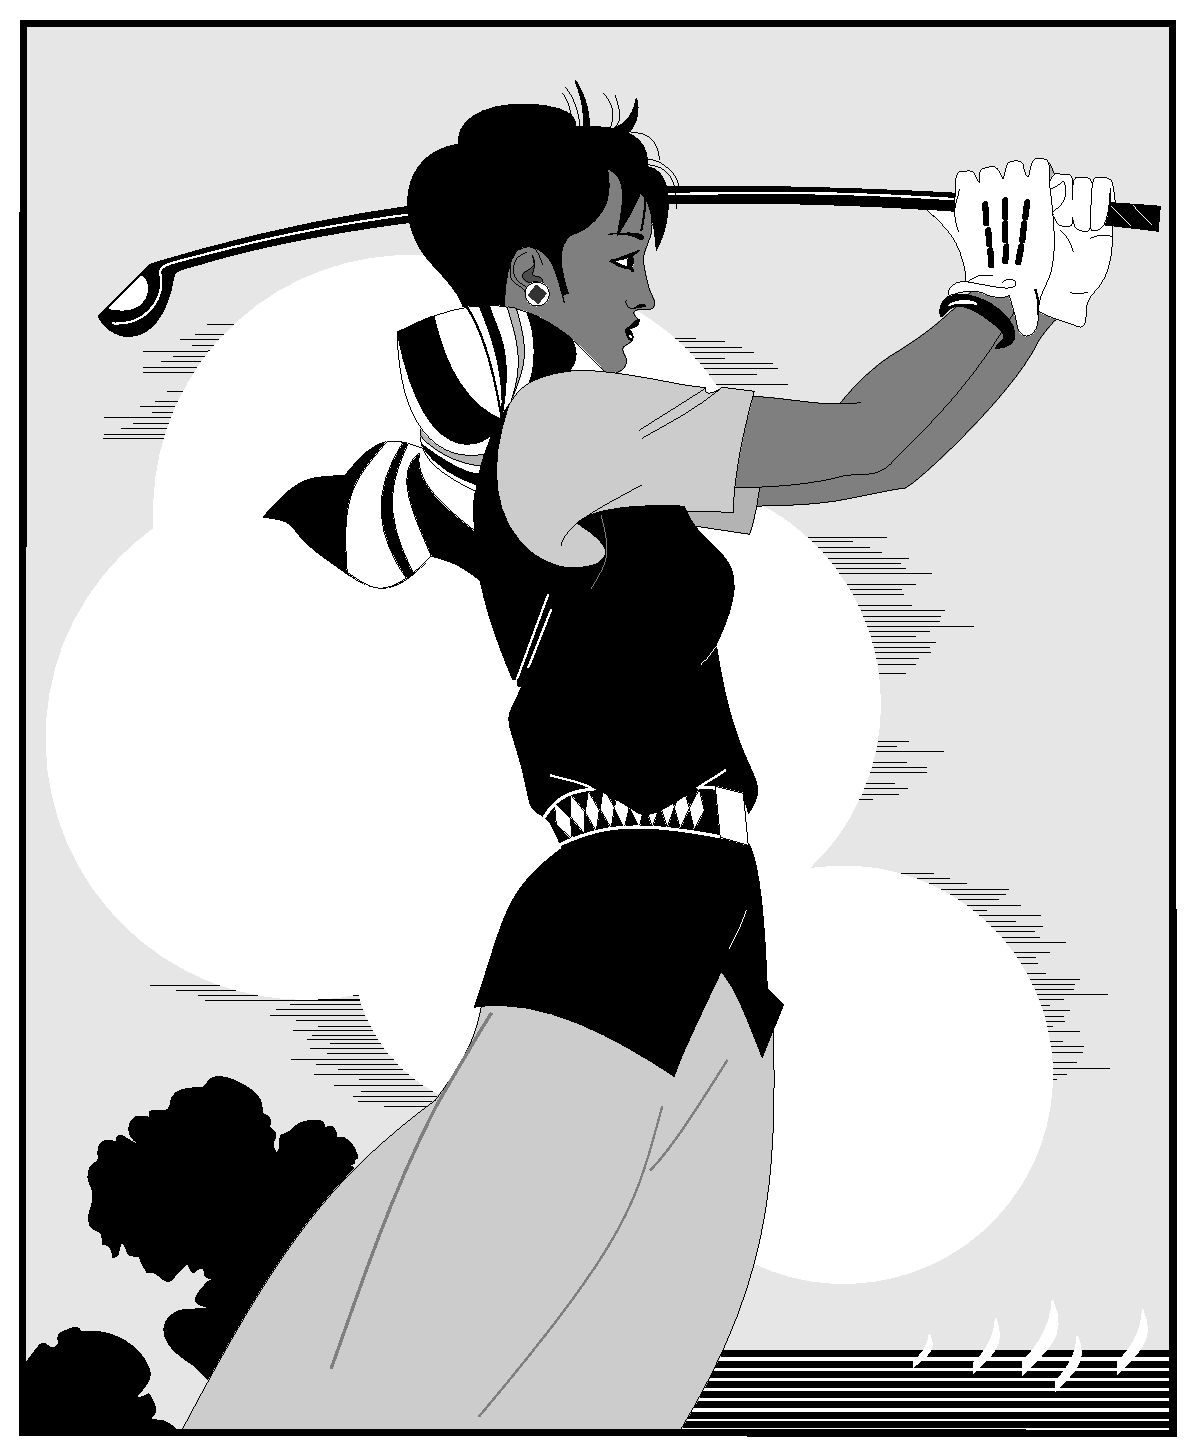
\includegraphics[width=0.4\textwidth]{golfer}}}
% \subfigure{\label{golfer42}}\addtocounter{subfigure}{-2}
% \subfigure[The person playing golf]{\subfigure[打高尔夫球的人~2]{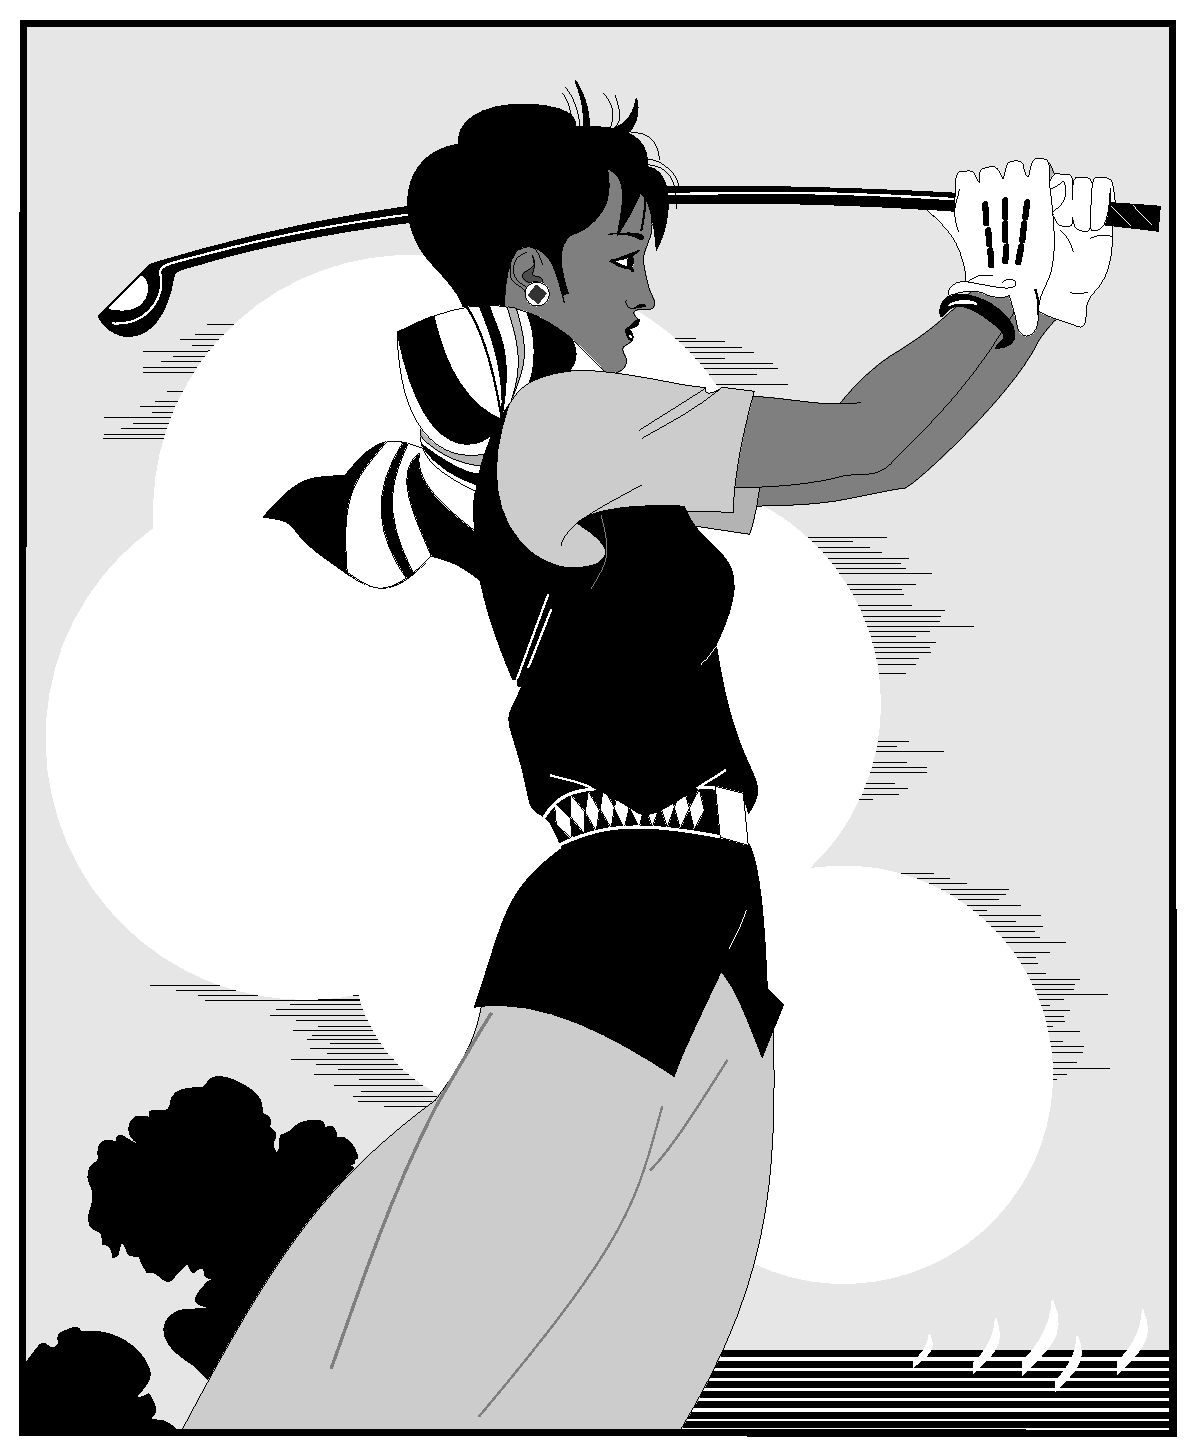
\includegraphics[width=0.4\textwidth]{golfer}}}
% \bicaption[golfer4]{}{打高尔夫球的人}{Fig.$\!$}{The person playing golf}
% \end{figure}
% \end{latex}
%
% 表格示例,表格中的字体是可以自行调整的:
% \begin{latex}
% \begin{table}[htbp]
% \bicaption[table1]{}{符合研究生院绘图规范的表格}{Table$\!$}{Table in agreement of the standard from graduate school}
% \vspace{0.5em}\centering\wuhao
% \begin{tabular}{ccccc}
% \toprule[1.5pt]
% $D$(in) & $P_u$(lbs) & $u_u$(in) & $\beta$ & $G_f$(psi.in)\\
% \midrule[1pt]
%  5 & 269.8 & 0.000674 & 1.79 & 0.04089\\
% 10 & 421.0 & 0.001035 & 3.59 & 0.04089\\
% 20 & 640.2 & 0.001565 & 7.18 & 0.04089\\
% \bottomrule[1.5pt]
% \end{tabular}
% \end{table}
% \end{latex}
%
% 因为长表格不是浮动体,不会自动调整位置、也不会自动调整字体大小,一切都要手动设
% 置。特别繁琐。长表格示例:
% \begin{latex}
% \ltfontsize{\dawu[1.667]} %设置表格内字体行间距
% \dawu[1.667]\begin{longtable}{ccc} % 注意此处设置的是表格线距离
% \longbionenumcaption{}{{\wuhao 中国省级行政单位一览 %此处要添加字体设置
% }\label{table2}}{Table$\!$}{}{{\wuhao Overview of the provincial administrative
% unit of China}}{-0.5em}{3.15bp}\\ %注意后两个参数分别是中英标题间距、标题和表格的间距。
% %\caption{\wuhao 中国省级行政单位一览}\\[1em] %注意此处是标题和表格间距,这行
% %是单语标题
% \toprule[1.5pt] 名称 & 简称 & 省会或首府  \\ \midrule[1pt]
% \endfirsthead
% \multicolumn{3}{r}{表~\thetable(续表)}\vspace{0.5em}\\
% \toprule[1.5pt] 名称 & 简称 & 省会或首府  \\ \midrule[1pt]
% \endhead
% \bottomrule[1.5pt]
% \endfoot
% 北京市 & 京 & 北京\\
% 天津市 & 津 & 天津\\
% 河北省 & 冀 & 石家庄市\\
% 山西省 & 晋 & 太原市\\
% 内蒙古自治区 & 蒙 & 呼和浩特市\\
% 辽宁省 & 辽 & 沈阳市\\
% 吉林省 & 吉 & 长春市\\
% 黑龙江省 & 黑 & 哈尔滨市\\
% 上海市 & 沪/申 & 上海\\
% 江苏省 & 苏 & 南京市\\
% 浙江省 & 浙 & 杭州市\\
% 安徽省 & 皖 & 合肥市\\
% 福建省 & 闽 & 福州市\\
% 江西省 & 赣 & 南昌市\\
% 山东省 & 鲁 & 济南市\\
% 河南省 & 豫 & 郑州市\\
% 湖北省 & 鄂 & 武汉市\\
% 湖南省 & 湘 & 长沙市\\
% 广东省 & 粤 & 广州市\\
% 广西壮族自治区 & 桂 & 南宁市\\
% 海南省 & 琼 & 海口市\\
% 重庆市 & 渝 & 重庆\\
% 四川省 & 川/蜀 & 成都市\\
% 贵州省 & 黔/贵 & 贵阳市\\
% 云南省 & 云/滇 & 昆明市\\
% 西藏自治区 & 藏 & 拉萨市\\
% 陕西省 & 陕/秦 & 西安市\\
% 甘肃省 & 甘/陇 & 兰州市\\
% 青海省 & 青 & 西宁市\\
% 宁夏回族自治区 & 宁 & 银川市\\
% 新疆维吾尔自治区 & 新 & 乌鲁木齐市\\
% 香港特别行政区 & 港 & 香港\\
% 澳门特别行政区 & 澳 & 澳门\\
% 台湾省 & 台 & 台北市\\
% \end{longtable}\normalsize %注意这里要恢复正常字体
% \end{latex}
%
% \subsubsection{公式}
%
% 公式不做介绍,与正常用法一致。
%
% \subsubsection{数学环境}
% \label{sec:math}
%
% \hitszthesis\ 定义了常用的数学环境:
%
% \begin{center}
% \begin{tabular}{*{7}{l}}\toprule
%   axiom & theorem & definition & proposition & lemma & conjecture &\\
%   公理 & 定理 & 定义 & 命题 & 引理 & 猜想 &\\\midrule
%   proof & corollary & example & exercise & assumption & remark & problem \\
%   证明 & 推论 & 例子& 练习 & 假设 & 注释 & 问题\\\bottomrule
% \end{tabular}
% \end{center}
%
% 比如:
% \begin{latex}
% \begin{definition}
%   道千乘之国,敬事而信,节用而爱人,使民以时。
% \end{definition}
% \end{latex}
% 产生(自动编号):
% \medskip
%
% \noindent\framebox[\linewidth][l]{{\heiti 定义~1.1~~~} % {道千乘之国,敬事而信,节用而爱人,使民以时。}}
%
% \smallskip
% 列举出来的数学环境毕竟是有限的,如果想用\emph{胡说}这样的数学环境,那么可以定义:
% \begin{latex}
% \newtheorem{nonsense}{胡说}[chapter]
% \end{latex}
%
% 然后这样使用:
% \begin{latex}
% \begin{nonsense}
%   契丹武士要来中原夺武林秘笈。—— 慕容博
% \end{nonsense}
% \end{latex}
% 产生(自动编号):
%
% \medskip
% \noindent\framebox[\linewidth][l]{{\heiti 胡说~1.1~~~} % {契丹武士要来中原夺武林秘笈。—— 慕容博}}
% \subsubsection{算法}
% 窝工算法不在规范中要求且一千个评审老师有一千个算法格式喜好。详见
% \href{https://github.com/PlutoThesis/PlutoThesis}{PlutoThesis}
% 中的各个实验室算法喜好举例。
% \subsubsection{引用参考文献}
% \DescribeMacro{\inlinecite}
% 学校要求的参考文献引用有两种模式:(1)上标模式。比如``同样的工作有很
% 多$^{[1,2]}$\ldots''。(2)正文模式。比如``文[3] 中详细说明了\ldots''。其中上标
% 模式使用远比正文模式频繁,所以为了符合使用习惯,上标模式仍然用常规
% 的 \cs{cite}\marg{key},而 \cs{inlinecite}\marg{key} 则用来生成正文模式。
%
% 关于参考文献模板推荐使用 \BibTeX,关于中文参考文献需要额外增加一个 Entry:
% \texttt{language},将其设置为 \texttt{zh} 用来指示此参考文献为中文,以
% 便 \file{hitszthesis.bst} 处理。如:
% \begin{latex}
% @INPROCEEDINGS{cnproceed,
%   author    = {王重阳 and 黄药师 and 欧阳峰 and 洪七公 and 段皇帝},
%   title     = {武林高手从入门到精通},
%   booktitle = {第~$N$~次华山论剑},
%   year      = 2006,
%   address   = {西安, 中国},
%   month     = sep,
%   language      = "zh",
% }
%
% @ARTICLE{cnarticle,
%   AUTHOR  = "贾宝玉 and 林黛玉 and 薛宝钗 and 贾探春",
%   TITLE   = "论刘姥姥食量大如牛之现实意义",
%   JOURNAL = "红楼梦杂谈",
%   PAGES   = "260--266",
%   VOLUME  = "224",
%   YEAR    = "1800",
%   LANGUAGE    = "zh",
% }
% \end{latex}
%
% 注意如果不需要引用参考文献,请删除 \file{main.tex} 中 \cs{bibliography} 开头的两行,
% 以避免可能的编译错误。
%
% \subsubsection{列表环境}
% \DescribeEnv{itemize}
% \DescribeEnv{enumerate}
% \DescribeEnv{description}
% 为了适合中文习惯,模板将这三个常用的列表环境用 \pkg{enumitem} 进行了纵向间距压
% 缩。一方面清除了多余空间,另一方面用户可以自己指定列表环境的样式(如标签符号,
% 缩进等)。细节请参看 \pkg{enumitem} 文档,此处不再赘述。
% \subsection{后文}
%
% \subsubsection{结论}
% \DescribeEnv{conclusion}
% 结论之后为后文内容。
%
% \lstinputlisting[style=lstStyleLaTeX]{back/conclusion.tex}
%
% \subsubsection{参考文献}
% 在后文中的参考文献是自动生成的,不需要用户干预,具体命令在\file{main.tex} 中有
% 示例。
%
% \subsubsection{附录}
% \DescribeEnv{appendix}
% 所有的附录都插到这里来。因为附录会更改默认的 chapter 属性,而后面的{\heiti 个人简
%   历}又需要恢复,所以实现为环境可以保证全局的属性不受影响。
% \begin{latex}
% \begin{appendix}
% \input{back/appA.tex}
% \end{appendix}
% \end{latex}
%
% \subsubsection{所发表文章}
% \DescribeEnv{publication}
% \PGR 与\UGR\ 中都没有明确规定此处的格式,以下仅为示例。
%
% \lstinputlisting[style=lstStyleLaTeX]{back/publications.tex}
%
% \subsubsection{索引}
% \DescribeEnv{ceindex}
% 窝工要求中英文双语索引。后文中的自动索引实际上不需要用户干预。
% \subsubsection{授权}
% \DescribeMacro{\authorization}
% 授权页中的签名和日期是需要手写,不需要人工干预。具体示例在\file{main.tex} 中。
%\begin{latex}
% \authorization %授权
% %\authorization[scan.pdf] %添加扫描页的命令,与上互斥
%\end{latex}
%
% \subsubsection{致谢声明}
% \DescribeEnv{acknowledgement}
% 把致谢做成一个环境更好一些,直接往里面写感谢的话就可以啦!
%
% \lstinputlisting[style=lstStyleLaTeX]{back/acknowledgements.tex}
%
% \subsubsection{简历}
% \DescribeEnv{resume}
% 个人简历。
% 实际上,致谢和个人简历是自由发挥的地区,字体,文体,格式,内容,完全自己决定。
%
% \lstinputlisting[style=lstStyleLaTeX]{back/resume.tex}
%
% \subsection{其它}
% 模板的配置文件 \file{hitszthesis.cfg} 中定义了很多固定词汇,一般无须修改。如果有特殊需求,
% 推荐在导言区使用 \cs{renewcommand}。
%
% \section{致谢}
% \label{sec:thanks}
% 感谢\href{https://github.com/dustincys/hithesis}{hithesis}、\href{https://github.com/xueruini/thuthesis}{thuthesis}模板的作者,本模板基于他们改编而来!
%
% 欢迎各位到 \href{http://github.com/YangLaTeX/hitszthesis/}{\hitszthesis\ Github 主页}贡献!
%
% \StopEventually{\PrintChanges\PrintIndex}
% \clearpage
%
% \section{实现细节}
%
% \subsection{基本信息}
%    \begin{macrocode}
%<cls>\NeedsTeXFormat{LaTeX2e}[1999/12/01]
%<cls>\ProvidesClass{hitszthesis}
%<cfg>\ProvidesFile{hitszthesis.cfg}
%<cls|cfg>[2020/03/10 3.0 Dissertation Template for Harbin Institute of Technology, ShenZhen (HITSZ)]
%    \end{macrocode}
%
% \subsection{定义选项}
% \label{sec:defoption}
%    \begin{macrocode}
%<*cls>
\RequirePackage{ifthen}
\RequirePackage{kvoptions}
\SetupKeyvalOptions{
  family=hitsz,
  prefix=hitsz@,
  setkeys=\kvsetkeys}
\newif\ifhitsz@bachelor
\newif\ifhitsz@master
\newif\ifhitsz@doctor
\define@key{hitsz}{type}{%
  \hitsz@bachelorfalse
  \hitsz@masterfalse
  \hitsz@doctorfalse
  \expandafter\csname hitsz@#1true\endcsname}
%    \end{macrocode}
%
% 此处设置校区,没有明确给出哈尔滨或者威海校区的时候,默认为深圳校区。
%    \begin{macrocode}
\newif\ifhitsz@shenzhen
\newif\ifhitsz@weihai
\newif\ifhitsz@harbin
\define@key{hitsz}{campus}{%
  \hitsz@shenzhenfalse
  \hitsz@weihaifalse
  \hitsz@harbinfalse
  \expandafter\csname hitsz@#1true\endcsname}
\ifhitsz@harbin
  \relax
\else
  \ifhitsz@weihai
    \relax
  \else
    \hitsz@shenzhentrue
  \fi
\fi
%    \end{macrocode}
%
% 目录中英文是否用 Arial 字体(默认关闭)。
%    \begin{macrocode}
\DeclareBoolOption[false]{arialtoc}
%    \end{macrocode}
%
% 章节标题中的英文是否用 Arial 字体(默认关闭)。
%    \begin{macrocode}
\DeclareBoolOption[false]{arialtitle}
%    \end{macrocode}
%
% 封面第二页信息是否居左对齐(默认关闭)。
%    \begin{macrocode}
\DeclareBoolOption[false]{infoleft}
%    \end{macrocode}
%
% 封面第一页标题是否为两行,如果标题过长可以选择(默认关闭)。
%    \begin{macrocode}
\DeclareBoolOption[false]{covertitletworow}
%    \end{macrocode}
%
% 图表题注是否加粗(默认关闭)。
%    \begin{macrocode}
\DeclareBoolOption[false]{boldcaption}
%    \end{macrocode}
%
% \option{raggedbottom} 选项(默认开启)。如果不开启这个选项,会出现一页中尽量上
% 下对齐,段的间距大。如果开启,尽量使段间距保持一致,页面底部出现空白。
%    \begin{macrocode}
\DeclareBoolOption[true]{raggedbottom}
%    \end{macrocode}
%
% 在脚注标记中使用 \pkg{pifont} 的带圈数字(默认关闭)。
%    \begin{macrocode}
\DeclareBoolOption[false]{pifootnote}
%    \end{macrocode}
%
% 字体间距设置(默认关闭)。
%    \begin{macrocode}
\DeclareBoolOption[false]{glue}
%    \end{macrocode}
%
% 文科生四级目录设置(默认关闭)。
%    \begin{macrocode}
\DeclareBoolOption[false]{tocfour}
%    \end{macrocode}
%
% 目录中“目录”位置是否空行(默认开启)。
%    \begin{macrocode}
\DeclareBoolOption[false]{tocblank}
%    \end{macrocode}
%
% 章标题是否悬挂居中(默认开启)
%    \begin{macrocode}
\DeclareBoolOption[true]{chapterhang}
%    \end{macrocode}
%
% 是否是全日制学生(默认是)。
%    \begin{macrocode}
\DeclareBoolOption[true]{fulltime}
%    \end{macrocode}
%
% 是否有子标题(默认是)。
%    \begin{macrocode}
\DeclareBoolOption[false]{subtitle}
%    \end{macrocode}
%
% 是否开启debug模式(默认否)。如果开启,载入显示行号等的包,只为开发调试用。
%    \begin{macrocode}
\DeclareBoolOption[false]{debug}
%    \end{macrocode}
%
% 是否使用右开页(默认否)。
%    \begin{macrocode}
\DeclareBoolOption[false]{openright}
%    \end{macrocode}
%
% 是否为提交图书馆电子版。
%    \begin{macrocode}
\DeclareBoolOption[false]{library}
%    \end{macrocode}
%
% 图题和标题最后一行是否居中对其(默认是,非规范要求)。
%    \begin{macrocode}
\DeclareBoolOption[true]{capcenterlast}
%    \end{macrocode}
%
% 子图图题和标题最后一行是否居中对其(默认是,非规范要求)。
%    \begin{macrocode}
\DeclareBoolOption[true]{subcapcenterlast}
%    \end{macrocode}
%
% 中文目录中Abstract是否均为大写
%    \begin{macrocode}
\DeclareBoolOption[true]{absupper}
%    \end{macrocode}
%
%    此处添加控制本科论文的页码横线选项
%    \begin{macrocode}
\DeclareBoolOption[true]{bsmainpagenumberline}
\DeclareBoolOption[true]{bsfrontpagenumberline}
\DeclareBoolOption[true]{bsheadrule}
%    \end{macrocode}
%
%    数学字体选项,默认使用\option{newtxmath}
%    \begin{macrocode}
\newif\ifhitsz@newtxmath
\newif\ifhitsz@mtprotwolite
\newif\ifhitsz@mtprotwo
\define@key{hitsz}{mathfont}{%
  \hitsz@newtxmathfalse
  \hitsz@mtprotwolitefalse
  \hitsz@mtprotwofalse
  \expandafter\csname hitsz@#1true\endcsname}
\ifhitsz@mtprotwolite
  \relax
\else
  \ifhitsz@mtprotwo
    \relax
  \else
    \hitsz@newtxmathtrue
  \fi
\fi
%    \end{macrocode}
%
%    参考文献分割开关
%    \begin{macrocode}
\DeclareBoolOption[false]{splitbibitem}
%    \end{macrocode}
%
% 声明字体选项
%    \begin{macrocode}
\DeclareStringOption{fontset}
%    \end{macrocode}
%
% 将其余选项默认传递给 \pkg{ctexbook}。
%    \begin{macrocode}
\DeclareDefaultOption{\PassOptionsToClass{\CurrentOption}{ctexbook}}
%    \end{macrocode}
%
% 解析用户传递过来的选项,并加载 \pkg{ctexbook}。
%    \begin{macrocode}
\ProcessKeyvalOptions*
%    \end{macrocode}
%
% 使用 \XeTeX\ 引擎时,\pkg{fontspec} 宏包会被 \pkg{xeCJK} 自动调用。传递
% 给 \pkg{fontspec} 宏包 \option{no-math} 选项,避免部分数学符号字体自动调整
% 为 CMR。其他引擎下没有这个问题,这一行会被无视。
%    \begin{macrocode}
\PassOptionsToPackage{no-math}{fontspec}
%    \end{macrocode}
%
% 载入单双面打印设置,本、硕单面,博士双面。
%    \begin{macrocode}
\ifhitsz@bachelor
\PassOptionsToClass{oneside}{book}
\fi
\ifhitsz@master
\PassOptionsToClass{oneside}{book}
\fi
\ifhitsz@doctor
\PassOptionsToClass{twoside}{book}
\fi
%    \end{macrocode}
%
% 设置字体。由于宋体没有粗体,且窝工模板的标题要求使用粗宋体,于是面临CTeX的经典
% 的伪粗体bug:“首次出现伪粗体字体之后的正常字体无法复制”。但如果使用自带宋体的
% 思源字体,那么不必使用伪粗体。模板只给出了新windows字体的思源字体设置,且思源
% 字体版本为Adobe版。
%    \begin{macrocode}
\ifthenelse%
{\equal{\hitsz@fontset}{}}%
{%
  \PassOptionsToPackage{AutoFakeBold=2}{xeCJK}
}%
{%
  \ifthenelse%
  {\equal{\hitsz@fontset}{siyuan}}%
  {\relax}%
  {%
    \PassOptionsToPackage{AutoFakeBold=2}{xeCJK}
  }%
  \PassOptionsToClass{fontset=\hitsz@fontset}{ctexbook}
}%
%    \end{macrocode}
%
% 使用 \XeLaTeX 编译 \pkg{mtpro2} 宏包必须加载此宏包
%    \begin{macrocode}
\RequirePackage{etex}
%    \end{macrocode}
%
% 使用 \pkg{ctexbook} 类,优于调用 \pkg{ctex} 宏包。
%    \begin{macrocode}
\LoadClass[a4paper,openany,UTF8,zihao=-4,scheme=plain]{ctexbook}
%    \end{macrocode}
%
% 用户至少要提供一个选项,指定论文类型。
%    \begin{macrocode}
\ifhitsz@bachelor\relax\else
  \ifhitsz@master\relax\else
    \ifhitsz@doctor\relax\else
        \ClassError{hitszthesis}%
                   {Please specify thesis type in option: \MessageBreak
                    type=[bachelor | master | doctor]}{}
      \fi
  \fi
\fi
%    \end{macrocode}
%
% \subsection{装载宏包}
% \label{sec:loadpackage}
%
% 引用的宏包和相应的定义。
%    \begin{macrocode}
\RequirePackage{etoolbox}
\RequirePackage{ifxetex}
\ifxetex
\else
        \ClassError{hitszthesis}%
                   {Please use: \MessageBreak
                    xelatex}{}
\fi
\RequirePackage{xparse}
%    \end{macrocode}
%
% \AmSTeX\ 宏包,用来排出更加漂亮的公式。
%    \begin{macrocode}
\RequirePackage{amsmath}
%    \end{macrocode}
%
% 定理类环境宏包,其中 \pkg{amsmath} 选项用来兼容 \AmSTeX\ 的宏包
%    \begin{macrocode}
\RequirePackage[amsmath,thmmarks,hyperref]{ntheorem}
\RequirePackage{amssymb}
%    \end{macrocode}
%
% \pkg{newtx} 设置 Times New Roman,Helvetica。
%    \begin{macrocode}
\RequirePackage[defaultsups]{newtxtext}
%    \end{macrocode}
%
% 添加数学字体开关
%    \begin{macrocode}
\ifhitsz@newtxmath
  \RequirePackage{newtxmath}
\else
  \ifhitsz@mtprotwolite
    \let\Bbbk\relax
    \RequirePackage[lite,subscriptcorrection,slantedGreek,nofontinfo]{mtpro2}
  \else
    \ifhitsz@mtprotwo
      \let\Bbbk\relax
      \RequirePackage[mtphrb,mtpcal,zswash,uprightGreek]{mtpro2}
    \fi
  \fi
\fi
%    \end{macrocode}
%
% 图形支持宏包。
%    \begin{macrocode}
\RequirePackage{graphicx}
%    \end{macrocode}
%
% \pkg{pdfpages} 宏包便于我们插入扫描后的授权页和声明页 PDF 文档。
%    \begin{macrocode}
\RequirePackage{pdfpages}
\includepdfset{fitpaper=true}
%    \end{macrocode}
%
% 更好的列表环境。
%    \begin{macrocode}
\RequirePackage{enumitem}  %使用enumitem宏包,改变列表项的格式
\RequirePackage{environ}
%    \end{macrocode}
%
% 禁止 \LaTeX 自动调整多余的页面底部空白,并保持脚注仍然在底部。
% 脚注按页编号。
%    \begin{macrocode}
\ifhitsz@raggedbottom
  \RequirePackage[bottom,perpage,hang]{footmisc}
  \raggedbottom
\else
  \RequirePackage[perpage,hang]{footmisc}
\fi
%    \end{macrocode}
%
% 脚注格式。
%    \begin{macrocode}
\ifhitsz@pifootnote
  \RequirePackage{pifont}
\fi
%    \end{macrocode}
%
% 利用 \pkg{CJKfntef} 实现汉字的下划线和盒子内两段对齐,并可以避免
% \cs{makebox}\oarg{width}\oarg{s} 可能产生的 underful boxes。
%    \begin{macrocode}
\RequirePackage{CJKfntef}
%    \end{macrocode}
%
% 表格控制
%    \begin{macrocode}
\RequirePackage{longtable}
%    \end{macrocode}
%
% 使用三线表:\cs{toprule},\cs{midrule},\cs{bottomrule}。
%    \begin{macrocode}
\RequirePackage{booktabs}
%    \end{macrocode}
%
% 参考文献引用宏包。
%    \begin{macrocode}
\RequirePackage[sort&compress]{natbib}
%    \end{macrocode}
%
% 子公式编号。
%    \begin{macrocode}
\RequirePackage{subeqnarray}
%    \end{macrocode}
%
% 生成有书签的 pdf 及其开关,请结合 gbk2uni 避免书签乱码。
%    \begin{macrocode}
\RequirePackage{hyperref}
\hypersetup{%
  CJKbookmarks=true,
  linktoc=all,
  bookmarksnumbered=true,
  bookmarksopen=true,
  bookmarksopenlevel=3,
  pdfcreator={XeLaTeX with hitszthesis class},
  breaklinks=true,
  colorlinks=false,
  plainpages=false,
  pdfstartview=FitH,
  pdfborder={0 0 0}
}
%    \end{macrocode}
%
% 设置 url 样式,与上下文一致
%    \begin{macrocode}
\urlstyle{same}
%    \end{macrocode}
%
% \subsection{页面设置}
% \label{sec:layout}
% 根据撰写规范设置版芯。
%    \begin{macrocode}
\ifhitsz@debug
  \RequirePackage[showframe]{geometry}
\else
  \RequirePackage{geometry}
\fi
\geometry{
  a4paper, % 210 * 297mm
  hcentering,
  ignoreall,
  nomarginpar,
}
%    \end{macrocode}
%
% 设置版芯页边距
%    \begin{macrocode}
\geometry{% 版芯高度 = textheight(224) + head(5) + headsep(3) + footskip(8) = 240 mm
  text={150true mm,224true mm},
  top=37.5true mm,
  left=30true mm,
  head=5true mm,
  headsep=3true mm,
  footskip=0true mm,
  foot=8true mm
}
%    \end{macrocode}
%
%    载入显示行号的包。
%    \begin{macrocode}
\ifhitsz@debug%
\RequirePackage{layout}
\RequirePackage{layouts}
\RequirePackage{lineno}
\fi
%    \end{macrocode}
%
% 利用 \pkg{fancyhdr} 设置页眉页脚。
%    \begin{macrocode}
\RequirePackage{fancyhdr}
%    \end{macrocode}
%
% 其他包,表格、数学符号包
%    \begin{macrocode}
\RequirePackage{tabularx}
\RequirePackage{varwidth}
%    \end{macrocode}
%
% 此处changepage环境用来控制索引页面的左右边距,规范中给出的示例的边距要大于正文。
%    \begin{macrocode}
\RequirePackage{changepage}
\RequirePackage{multicol}
\RequirePackage[below]{placeins}%允许上一个section的浮动图形出现在下一个section的开始部分,还提供\FloatBarrier命令,使所有未处理的浮动图形立即被处理
\RequirePackage{flafter}       % 使得所有浮动体不能被放置在其浮动环境之前,以免浮动体在引述它的文本之前出现.
\RequirePackage{multirow}       %使用Multirow宏包,使得表格可以合并多个row格
\ifhitsz@subcapcenterlast
\PassOptionsToPackage{centerlast}{subfigure}
\fi
\RequirePackage{subfigure}%支持子图 %centerlast 设置最后一行是否居中
\RequirePackage[subfigure]{ccaption} %支持双语标题
%    \end{macrocode}
%
%    中英文索引包。
%    \begin{macrocode}
\RequirePackage[makeindex]{splitidx}
\newindex[]{china}
\newindex[]{english}
%</cls>
%    \end{macrocode}
%
%    窝工要求的索引格式。
%    \begin{macrocode}
%<*ist>
headings_flag 1
heading_prefix "\{\\vskip -\\baselineskip\\centering\\normalsize\\textbf\{"
heading_suffix "\}\\par\}\\nopagebreak\\wuhao\n"
delim_0 "\\hspace*{\\fill}"
delim_1 "\\hspace*{\\fill}"
%</ist>
%    \end{macrocode}
%
%    排版logo。
%    \begin{macrocode}
%<cls>\RequirePackage{xltxtra}
%    \end{macrocode}
%
% \subsection{主文档格式}
% \label{sec:mainbody}
%
% \subsubsection{Three matters}
%
% \begin{macro}{\cleardoublepage}
% 对于 \textsl{openright} 选项,必须保证章首页右开,且如果前章末页无内容须
% 清空其页眉页脚。
% 如果\textsl{library}为真,则强制设置\textsl{openright}为真。
%    \begin{macrocode}
%<*cls>
\ifhitsz@library
  \hitsz@openrightfalse
\else
  \relax
\fi
\let\hitsz@cleardoublepage\cleardoublepage
\newcommand{\hitsz@clearemptydoublepage}{%
  \clearpage{\pagestyle{hitsz@empty}\hitsz@cleardoublepage}
}
\let\cleardoublepage\hitsz@clearemptydoublepage
%    \end{macrocode}
% \end{macro}
%
% \begin{macro}{\frontmatter}
% 我们的单面和双面模式与常规的不太一样。
%    \begin{macrocode}
\renewcommand\frontmatter{%
  \ifhitsz@openright\cleardoublepage\else\clearpage\fi
  \@mainmatterfalse
  \pagenumbering{Roman}
  \pagestyle{hitsz@empty}
}
%    \end{macrocode}
% \end{macro}
%
% \begin{macro}{\mainmatter}
% 根据打印店(伪官方)的猛虎式操作,\cs{mainmatter}命令的逻辑是,双面打印时第一章必须在奇数页。
%    \begin{macrocode}
\renewcommand\mainmatter{%
  \ifhitsz@tocblank%
  \addtocontents{toc}{\vspace{\baselineskip}}
  \addtocontents{toe}{\vspace{\baselineskip}}
  \fi%
  \ifhitsz@doctor%
    \ifhitsz@library\clearpage\else\cleardoublepage\fi
    \else%
    \clearpage
  \fi%
  \@mainmattertrue
  \pagenumbering{arabic}
  \pagestyle{hitsz@headings}
}
%    \end{macrocode}
% \end{macro}
% \begin{macro}{\backmatter}
%    \begin{macrocode}
\renewcommand\backmatter{%
  \ifhitsz@openright\cleardoublepage\else\clearpage\fi
  \@mainmattertrue}
%</cls>
%    \end{macrocode}
% \end{macro}
%
% \subsubsection{字体}
% \label{sec:font}
%
% \begin{macro}{\normalsize}
% 根据窝工规定,正文小四号 (12bp) 字,行距为1.25倍。
%    \begin{macrocode}
%<*cls>
\renewcommand\normalsize{%
  \@setfontsize\normalsize{12bp}{ \ifhitsz@glue 20.50398bp \@plus 2.83465bp \@minus 0bp
                                  \else 19.27374bp
                                  \fi}%
  \abovedisplayskip=8pt
  \abovedisplayshortskip=8pt
  \belowdisplayskip=\abovedisplayskip
  \belowdisplayshortskip=\abovedisplayshortskip}
%    \end{macrocode}
% \end{macro}
%
% WORD 中的字号对应该关系如下(1bp = 72.27/72 pt):
% \begin{center}
% \begin{tabular}{llll}
% \toprule
% 初号 & 42bp & 14.82mm & 42.1575pt \\
% 小初 & 36bp & 12.70mm & 36.135 pt \\
% 一号 & 26bp & 9.17mm & 26.0975pt \\
% 小一 & 24bp & 8.47mm & 24.09pt \\
% 二号 & 22bp & 7.76mm & 22.0825pt \\
% 小二 & 18bp & 6.35mm & 18.0675pt \\
% 三号 & 16bp & 5.64mm & 16.06pt \\
% 小三 & 15bp & 5.29mm & 15.05625pt \\
% 四号 & 14bp & 4.94mm & 14.0525pt \\
% 小四 & 12bp & 4.23mm & 12.045pt \\
% 五号 & 10.5bp & 3.70mm & 10.59375pt \\
% 小五 & 9bp & 3.18mm & 9.03375pt \\
% 六号 & 7.5bp & 2.56mm & \\
% 小六 & 6.5bp & 2.29mm & \\
% 七号 & 5.5bp & 1.94mm & \\
% 八号 & 5bp & 1.76mm & \\\bottomrule
% \end{tabular}
% \end{center}
%
% \begin{macro}{\hitsz@def@fontsize}
% 根据习惯定义字号。用法:\cs{hitsz@def@fontsize}\marg{字号名称}\marg{磅数}避免了
% 字号选择和行距的紧耦合。所有字号定义时为单倍行距,并提供选项指定行距倍数。
%    \begin{macrocode}
\def\hitsz@def@fontsize#1#2{%
  \expandafter\newcommand\csname #1\endcsname[1][1.3]{%
    \fontsize{#2}{##1\dimexpr #2}\selectfont}}
%    \end{macrocode}
% \end{macro}
%
% \begin{macro}{\dachu}
% \begin{macro}{\chuhao}
% \begin{macro}{\xiaochu}
% \begin{macro}{\yihao}
% \begin{macro}{\xiaoyi}
% \begin{macro}{\erhao}
% \begin{macro}{\xiaoer}
% \begin{macro}{\sanhao}
% \begin{macro}{\xiaosan}
% \begin{macro}{\sihao}
% \begin{macro}{\banxiaosi}
% \begin{macro}{\xiaosi}
% \begin{macro}{\dawu}
% \begin{macro}{\wuhao}
% \begin{macro}{\xiaowu}
% \begin{macro}{\liuhao}
% \begin{macro}{\xiaoliu}
% \begin{macro}{\qihao}
% \begin{macro}{\bahao}
% 一组字号定义。
%    \begin{macrocode}
\hitsz@def@fontsize{dachu}{58bp}
\hitsz@def@fontsize{chuhao}{42bp}
\hitsz@def@fontsize{xiaochu}{36bp}
\hitsz@def@fontsize{yihao}{26bp}
\hitsz@def@fontsize{xiaoyi}{24bp}
\hitsz@def@fontsize{erhao}{22bp}
\hitsz@def@fontsize{xiaoer}{18bp}
\hitsz@def@fontsize{sanhao}{16bp}
\hitsz@def@fontsize{xiaosan}{15bp}
\hitsz@def@fontsize{sihao}{14bp}
\hitsz@def@fontsize{banxiaosi}{13bp}
\hitsz@def@fontsize{xiaosi}{12bp}
\hitsz@def@fontsize{dawu}{11bp}
\hitsz@def@fontsize{wuhao}{10.5bp}
\hitsz@def@fontsize{xiaowu}{9bp}
\hitsz@def@fontsize{liuhao}{7.5bp}
\hitsz@def@fontsize{xiaoliu}{6.5bp}
\hitsz@def@fontsize{qihao}{5.5bp}
\hitsz@def@fontsize{bahao}{5bp}
%</cls>
%    \end{macrocode}
% \end{macro}
% \end{macro}
% \end{macro}
% \end{macro}
% \end{macro}
% \end{macro}
% \end{macro}
% \end{macro}
% \end{macro}
% \end{macro}
% \end{macro}
% \end{macro}
% \end{macro}
% \end{macro}
% \end{macro}
% \end{macro}
% \end{macro}
% \end{macro}
% \end{macro}
%
% \subsubsection{页眉页脚}
% \label{sec:headerfooter}
%
% \begin{macro}{\hitsz@empty}
% \begin{macro}{\hitsz@plain}
% \begin{macro}{\hitsz@headings}
% 定义三种页眉页脚格式:
% \begin{itemize}
% \item \texttt{hitsz@empty}:页眉页脚都没有
% \item \texttt{hitsz@plain}:只显示页脚的页码。\cs{chapter} 自动调用
% \cs{thispagestyle\{hitsz@plain\}}。
% \item \texttt{hitsz@headings}:页眉页脚同时显示
% \end{itemize}
%    \begin{macrocode}
%<*cls>
\let\hitsz@headrule\headrule
\fancypagestyle{hitsz@empty}{%
  \fancyhf{}
  \let\headrule\hitsz@headrule%
  \renewcommand{\headrulewidth}{0pt}
  \renewcommand{\footrulewidth}{0pt}
}
%    \end{macrocode}
%
%    此处根据本科生模板的多种版本,提供选项自定义页码、页眉样式。
%    \begin{macrocode}
\fancypagestyle{hitsz@headings}{%
  \fancyhf{}
  \ifhitsz@doctor
    \fancyhead[CO]{\songti\xiaowu[0]\leftmark}
    \ifhitsz@harbin
      \fancyhead[CE]{\songti\xiaowu[0]\hitsz@cschoolname\hitsz@cdegree\hitsz@cthesisname}
    \fi
    \ifhitsz@shenzhen
      \fancyhead[CE]{\songti\xiaowu[0]%
        \hitsz@cschoolname\hitsz@cdegree\hitsz@cthesisname}
    \fi
    \ifhitsz@weihai
      \fancyhead[CE]{\songti\xiaowu[0]%
        \hitsz@cschoolname\hitsz@weihaicampus\hitsz@cdegree\hitsz@cthesisname}
    \fi
  \else
    \ifhitsz@master
      \ifhitsz@harbin
        \fancyhead[C]{\songti\xiaowu[0]%
          \hitsz@cschoolname\hitsz@cdegree\hitsz@cthesisname}
      \fi
      \ifhitsz@shenzhen
        \fancyhead[C]{\songti\xiaowu[0]%
          \hitsz@cschoolname\hitsz@cdegree\hitsz@cthesisname}
      \fi
      \ifhitsz@weihai
        \fancyhead[C]{\songti\xiaowu[0]%
          \hitsz@cschoolname\hitsz@weihaicampus\hitsz@cdegree\hitsz@cthesisname}
      \fi
    \fi
  \fi
  \ifhitsz@bachelor
    \ifhitsz@harbin
      \fancyhead[C]{\songti\xiaowu[0]%
        \hitsz@cschoolname\hitsz@bachelor@cxuewei\hitsz@bachelor@cthesisname}%
    \fi
    \ifhitsz@shenzhen
      \fancyhead[C]{\songti\xiaowu[0]%
        \hitsz@cschoolname\hitsz@shenzhencampus\hitsz@bachelor@cxuewei\hitsz@bachelor@cthesisname}%
    \fi
    \ifhitsz@weihai
      \fancyhead[C]{\songti\xiaowu[0]%
        \hitsz@cschoolname\hitsz@weihaicampus\hitsz@bachelor@cxuewei\hitsz@bachelor@cthesisname}%
    \fi
    \fancyfoot[C]{\xiaowu%
      \if@mainmatter%
        \ifhitsz@bsmainpagenumberline-~\thepage~-
        \else\thepage
        \fi
      \else%
        \ifhitsz@bsfrontpagenumberline-~\thepage~-
        \else\thepage
        \fi
      \fi
    }
    \ifhitsz@bsheadrule
      \renewcommand{\headrule}{
        \vskip 1.190132pt
        \hrule\@height2.276208pt\@width\headwidth
        \vskip 0.75pt
        \hrule\@height.75pt\@width\headwidth
      }
    \else
      \renewcommand{\headrulewidth}{0pt}
    \fi
  \else%
    \fancyfoot[C]{\xiaowu-~\thepage~-}
    \renewcommand{\headrule}{%
      \vskip 1.190132pt
      \hrule\@height2.276208pt\@width\headwidth
      \vskip 0.75pt
      \hrule\@height.75pt\@width\headwidth
    }
  \fi
  % 页眉中小五汉字,0行距时,占用9bt,页眉高度为14pt,
  % 所以页眉中headrule四个距离之和要保持等于 14pt - 9bt = 4.96634pt
  \renewcommand{\footrulewidth}{0pt}
}
\AtBeginDocument{%此处解决页眉经典bug
  \pagestyle{hitsz@empty}
  \renewcommand{\chaptermark}[1]{\@mkboth{\CTEXthechapter\enspace#1}{}}}
%</cls>
%    \end{macrocode}
% \end{macro}
% \end{macro}
% \end{macro}
%
% \subsubsection{段落}
% \label{sec:paragraph}
%
% 全文首行缩进 2 字符,标点符号用全角
%    \begin{macrocode}
%<*cls>
\ctexset{%
  punct=quanjiao,
  space=auto,
  autoindent=true}
%    \end{macrocode}
%
% 利用 \pkg{enumitem} 命令调整默认列表环境间的距离,以符合中文习惯。
%    \begin{macrocode}
\setlist{nosep}
%</cls>
%    \end{macrocode}
%
% \subsubsection{脚注}
% \label{sec:footnote}
%
% 脚注符合中文习惯,数字带圈。
%    \begin{macrocode}
%<*cls>
\def\hitsz@textcircled#1{%
  \ifnum\value{#1} >9
    \ClassError{hitszszthesis}%
      {Too many footnotes in this page.}{Keep footnote less than 10.}
  \fi
  \ifhitsz@pifootnote%
    \ding{\the\numexpr\value{#1}+171\relax}%
  \else%
    \textcircled{\xiaoliu\arabic{#1}}%
  \fi}
\renewcommand{\thefootnote}{\hitsz@textcircled{footnote}}
\renewcommand{\thempfootnote}{\hitsz@textcircled{mpfootnote}}
%    \end{macrocode}
%
% 定义脚注分割线,字号(宋体小五),以及悬挂缩进(1.5字符)。
%    \begin{macrocode}
\def\footnoterule{\vskip-3\p@\hrule\@width0.3\textwidth\@height0.4\p@\vskip2.6\p@}
\let\hitsz@footnotesize\footnotesize
\renewcommand\footnotesize{\hitsz@footnotesize\xiaowu[1.5]}
\footnotemargin1.5em\relax
%    \end{macrocode}
%
% \cs{@makefnmark} 默认是上标样式,而在脚注部分要求为正文大小。利用\cs{patchcmd}
% 动态调整 \cs{@makefnmark} 的定义。
%    \begin{macrocode}
\let\hitsz@makefnmark\@makefnmark
\def\hitsz@@makefnmark{\hbox{{\normalfont\@thefnmark}}}
\pretocmd{\@makefntext}{\let\@makefnmark\hitsz@@makefnmark}{}{}
\apptocmd{\@makefntext}{\let\@makefnmark\hitsz@makefnmark}{}{}
%</cls>
%    \end{macrocode}
%
% \subsubsection{数学相关}
% \label{sec:equation}
%
% 允许太长的公式断行、分页等。
%    \begin{macrocode}
%<*cls>
\allowdisplaybreaks[4]
\predisplaypenalty=0  %公式之前可以换页,公式出现在页面顶部
\postdisplaypenalty=0
\renewcommand\theequation{\ifnum \c@chapter>\z@ \thechapter-\fi\@arabic\c@equation}
%    \end{macrocode}
%
% 公式距前后文的距离由 4 个参数控制,参见 \cs{normalsize} 的定义。
% 同时为了让 \pkg{amsmath} 的 \cs{tag*} 命令得到正确的格式,我们必须修改这些代
% 码。\cs{make@df@tag} 是定义 \cs{tag*} 和 \cs{tag} 内部命令的。
% \cs{make@df@tag@@} 处理 \cs{tag*},我们就改它!
% \begin{latex}
% \def\make@df@tag{\@ifstar\make@df@tag@@\make@df@tag@@@}
% \def\make@df@tag@@#1{%
%   \gdef\df@tag{\maketag@@@{#1}\def\@currentlabel{#1}}}
% \end{latex}
%    \begin{macrocode}
\def\make@df@tag{\@ifstar\hitsz@make@df@tag@@\make@df@tag@@@}
\def\hitsz@make@df@tag@@#1{\gdef\df@tag{\hitsz@maketag{#1}\def\@currentlabel{#1}}}
\iffalse
\ifhitsz@bachelor
  \def\hitsz@maketag#1{\maketag@@@{%
    (\ignorespaces\text{\equationname\hskip0.5em}#1\unskip\@@italiccorr)}}
  \def\tagform@#1{\maketag@@@{%
    (\ignorespaces\text{\equationname\hskip0.5em}#1\unskip\@@italiccorr)\equcaption{#1}}}
\fi
\fi
\def\hitsz@maketag#1{\maketag@@@{(\ignorespaces #1\unskip\@@italiccorr)}}
\def\tagform@#1{\maketag@@@{(\ignorespaces #1\unskip\@@italiccorr)\equcaption{#1}}}
%    \end{macrocode}
%
% 修改 \cs{tagform} 会影响 \cs{eqref}。
%    \begin{macrocode}
\renewcommand{\eqref}[1]{\textup{(\ref{#1})}}
%</cls>
%    \end{macrocode}
%
% 定理标题使用黑体,正文使用宋体,冒号隔开。
%    \begin{macrocode}
%<*cfg>
\theorembodyfont{\normalfont}
\theoremheaderfont{\normalfont\heiti}
\theoremsymbol{\ensuremath{\square}}
\newtheorem*{proof}{证明}
\theoremstyle{plain}
\theoremsymbol{}
%    \end{macrocode}
%
% 此处去除了冒号,如果需要在加上这个冒号。
%    \begin{macrocode}
\theoremseparator{}
\newtheorem{assumption}{假设}[chapter]
\newtheorem{definition}{定义}[chapter]
\newtheorem{proposition}{命题}[chapter]
\newtheorem{lemma}{引理}[chapter]
\newtheorem{theorem}{定理}[chapter]
\newtheorem{axiom}{公理}[chapter]
\newtheorem{corollary}{推论}[chapter]
\newtheorem{exercise}{练习}[chapter]
\newtheorem{example}{例}[chapter]
\newtheorem{remark}{注释}[chapter]
\newtheorem{problem}{问题}[chapter]
\newtheorem{conjecture}{猜想}[chapter]
%</cfg>
%    \end{macrocode}
%
% \subsubsection{浮动对象以及表格}
% \label{sec:float}
%
% 设置浮动对象和文字之间的距离,由于规范中没有明确规定,根据经验,设置成正文汉字
% 高度。
%    \begin{macrocode}
%<*cls>
\setlength{\intextsep}{\ifhitsz@glue 8.50398bp \@plus 2.83465bp \@minus 0bp\else 8.50398bp\fi}
\setlength{\textfloatsep}{\ifhitsz@glue 8.50398bp \@plus 2.83465bp \@minus 0bp\else 8.50398bp\fi}
\setlength{\floatsep}{\ifhitsz@glue 12bp \@plus 2.83465bp \@minus 0bp\else 12bp\fi}
%    \end{macrocode}
%
%    此处设置float在p选项时间隔,此处不设置\cs{@fptop}和\cs{@fpbot}以确保居中。
% 下面这组命令使浮动对象的缺省值稍微宽松一点,从而防止幅度对象占据过多的文本页面,
% 也可以防止在很大空白的浮动页上放置很小的图形。
%    \begin{macrocode}
\g@addto@macro\appendix{\renewcommand*{\thefigure}{\thechapter-\arabic{figure}}}
\g@addto@macro\appendix{\renewcommand*{\thetable}{\thechapter-\arabic{table}}}
\g@addto@macro\appendix{\renewcommand*{\theequation}{\thechapter-\arabic{equation}}}
\renewcommand{\textfraction}{0.15}
\renewcommand{\topfraction}{0.85}
\renewcommand{\bottomfraction}{0.65}
\renewcommand{\floatpagefraction}{0.60}
%    \end{macrocode}
%
% 由于窝工的双标题,导致标题之下多出一空白字符的距离,去除。
%    \begin{macro}{\@makecaption}
%    根据窝工规范,本科和硕博的图题序号之后的空格不一样。
%    \begin{hitszrgu}[\PGR][2.13.1]
% 每个图均应有图题(由图序和图名组成),图题不宜有标点符号,图名在图序之后空1个
% 半角字符排写。
%    \end{hitszrgu}
%    \begin{hitszrgu}[\UGR][2.13.1]
% 每个图均应有图题(由图序和图名组成),图题不宜有标点符号,图名在图序之后空1个
% 字符排写。
%    \end{hitszrgu}
%    窝工规范中没有明确规定是否标题是否居中对齐,这里给出一个居中选项自行调整。
% 注意,窝工只规定:“居中书写”。此处不额外添加悬挂处理。
%    \begin{macrocode}
\long\def\@makecaption#1#2{%
  \vskip\abovecaptionskip
  \ifhitsz@boldcaption\songti\bfseries\fi
  \wuhao\sbox\@tempboxa{#1\ifhitsz@bachelor\hskip\ccwd\else\enskip\fi#2}%
  \ifdim \wd\@tempboxa >\hsize
	  \ifhitsz@capcenterlast%
		  \vskip 6.3bp%
		  {\setbox0=\vbox{#1\ifhitsz@bachelor\hskip\ccwd\else\enskip\fi#2}
			  \setbox1=\vbox{%
				  \unvbox0
				  \setbox2=\lastbox
				  \hbox to \textwidth{\hfill\unhcopy2 \unskip\unskip\hfill}
			  }
		  \unvbox1}
	  \else%
		  #1\ifhitsz@bachelor\hskip\ccwd\else\enskip\fi#2%
	  \fi%
    \par
  \else
    \global \@minipagefalse
    \hb@xt@\hsize{\hfil\box\@tempboxa\hfil}%
  \fi
\vskip\belowcaptionskip}
%    \end{macrocode}
%    \end{macro}
%
%    \begin{macro}{\longbionenumcaption}
% 长表格的双语标题是一个坑. 因为第一不能用浮动格式,只能用longtable包中的tabular
% ,这样表题只能使用表格中前两行来写。这样出现了一个问题是,中英表题的间距,标题
% 和表第一行间距,表格内部间距等多个变量的协调问题。这个问题只要使用tabular的形
% 式,就是无解的。唯一的方法就是把这些参数都给用户列出来。以下,第2,5参数为中英
% 双语标题内容,1,4为标题参数。6为中英标题间距,7为表题和表格间距。
%    \begin{macrocode}
\renewcommand*{\longbionenumcaption}[7]{%
\@if@contemptyarg{#1}{\caption{#2}}{\caption[#1]{#2}}%
\global\let\@cont@oldtablename\tablename
\gdef\tablename{#3}
\global\let\LT@c@ption\@cont@LT@nonumintoc
\\[#6]
\@if@contemptyarg{#4}{\caption{#5}}{\caption[#4]{#5}}%
\global\let\tablename\@cont@oldtablename
\global\let\LT@c@ption\@cont@oldLT@c@ption
\vspace{#7}}
%    \end{macrocode}
%    \end{macro}
%
%    \begin{macro}{\ltfontsize}
% 我们采用 \pkg{longtable} 来处理跨页的表格。同样我们需要设置其默认字体为五号,
% 行距设置为1.3倍行距。此处还需要提供一个设置长表格内部字体的命令。
%    \begin{macrocode}
\let\hitsz@LT@array\LT@array
\def\LT@array{\wuhao\hitsz@LT@array} % set default font size
\newcommand{\ltfontsize}[1]{\def\LT@array{#1\hitsz@LT@array}}
%    \end{macrocode}
%    \end{macro}
%
%    图表名称及格式。
%    \begin{macrocode}
\renewcommand{\thesubtable}{(\alph{subtable})}
\renewcommand{\thefigure}{\arabic{chapter}-\arabic{figure}}%使图编号为 7-1 的格式 %\protect{~}
\renewcommand{\thesubfigure}{\alph{subfigure})}%使子图编号为 a)的格式
\renewcommand{\p@subfigure}{\thefigure~} %使子图引用为 7-1 a) 的格式,母图编号和子图编号之间用~加一个空格
\renewcommand{\thetable}{\arabic{chapter}-\arabic{table}}%使表编号为 7-1 的格式
%    \end{macrocode}
%
% \begin{macro}{\figref}
% \begin{macro}{\tabref}
% \begin{macro}{\equref}
% 图表的引用格式
%    \begin{macrocode}
\newcommand\figref[1]{图\ref{#1}}
\newcommand\tabref[1]{表\ref{#1}}
\newcommand\equref[1]{式(\ref{#1})}
%    \end{macrocode}
% \end{macro}
% \end{macro}
% \end{macro}
%
%    调整罗列环境、浮动格式、间距。
%    \begin{macrocode}
\setitemize{leftmargin=0em,itemsep=0em,partopsep=0em,parsep=0em,topsep=0em,itemindent=3em}
\setenumerate{leftmargin=0em,itemsep=0em,partopsep=0em,parsep=0em,topsep=0em,itemindent=3.5em}
\newcommand{\citeup}[1]{\textsuperscript{\cite{#1}}}
%    \end{macrocode}
%
% 此处删除hang caption的设置
%    \begin{macrocode}
\captionnamefont{\wuhao}
\captiontitlefont{\wuhao}
\renewcommand{\subcapsize}{\wuhao}
\setlength{\abovecaptionskip}{0pt}%为了双标题之间的间距,不能设置
\setlength{\belowcaptionskip}{0pt}
% 自定义项目列表标签及格式 \begin{publist} 列表项 \end{publist}
\newcounter{pubctr} %自定义新计数器
\newenvironment{publist}{%%%%%定义新环境
\begin{list}{[\arabic{pubctr}]} %%标签格式
    {
     \usecounter{pubctr}
     \setlength{\leftmargin}{1.7em}     % 左边界 \leftmargin =\itemindent + \labelwidth + \labelsep
     \setlength{\itemindent}{0em}     % 标号缩进量
     \setlength{\labelsep}{0.5em}       % 标号和列表项之间的距离,默认0.5em
     \setlength{\rightmargin}{0em}    % 右边界
     \setlength{\topsep}{0ex}         % 列表到上下文的垂直距离
     \setlength{\parsep}{0ex}         % 段落间距
     \setlength{\itemsep}{0ex}        % 标签间距
     \setlength{\listparindent}{0pt} % 段落缩进量
    }}
{\end{list}}
%    \end{macrocode}
%
% 设置定理定义格式
%    \begin{macrocode}
\renewtheoremstyle{plain}
{\item[\hskip\labelsep \theorem@headerfont ##1\ ##2\theorem@separator]}
{\item[\hskip\labelsep \theorem@headerfont ##1\ ##2\ ##3\theorem@separator]}
\theorembodyfont{\songti\rmfamily}
\theoremheaderfont{\heiti\rmfamily}
\theoremsymbol{$\square$}
\setlength{\theorempreskipamount}{0pt}
\setlength{\theorempostskipamount}{-2pt}
\setlength{\parindent}{2em}
\arraycolsep=1.6pt
%</cls>
%    \end{macrocode}
%
% \subsubsection{章节标题}
% \label{sec:theor}
%
%    \begin{macrocode}
%<*cfg>
\ctexset{%
  chapter/name={第,章},
  appendixname=附录,
  contentsname={目\hspace{\ccwd}录},
  listfigurename=插图索引,
  listtablename=表格索引,
  figurename=图,
  tablename=表,
  bibname=参考文献,
  indexname=索引,
}
\newcommand\listfigureename{Index of figure}
\newcommand\listtableename{Index of table}
\newcommand\listequationename{Index of equation}
\newcommand\listequationname{公式索引}
\newcommand\equationname{公式}
\newcommand{\cabstractcname}{摘\hspace{\ccwd}要}
\newcommand{\cabstractename}{Abstract (In Chinese)}
%    \end{macrocode}
%
% 此处删除冗余选项
%    \begin{macrocode}
\newcommand{\eabstractcname}{Abstract}
\newcommand{\eabstractename}{Abstract (In English)}
\newcommand{\hitsz@ckeywords@title}{关键词:}
\def\hitsz@ckeywords@separator{;}
\def\hitsz@ekeywords@separator{,}
\let\CJK@todaysave=\today
\def\CJK@todaysmall@short{\the\year 年 \the\month 月}
\def\CJK@todaysmall{\the\year 年 \the\month 月 \the\day 日}
\def\CJK@todaybig@short{\zhdigits{\the\year}年\zhnumber{\the\month}月}
\def\CJK@todaybig{\zhdigits{\the\year}年\zhnumber{\the\month}月\zhnumber{\the\day}日}
\def\CJK@today{\CJK@todaysmall}
\renewcommand\today{\CJK@today}
\newcommand\CJKtoday[1][1]{%
  \ifcase#1\def\CJK@today{\CJK@todaysave}
    \or\def\CJK@today{\CJK@todaysmall}
    \or\def\CJK@today{\CJK@todaybig}
  \fi}
%    \end{macrocode}
%
% 按照word示范要求,此处使用阿拉伯数字
%    \begin{macrocode}
\cdate{\ifhitsz@bachelor\CJK@todaysmall@short\else\CJK@todaysmall@short\fi}
\edate{\ifcase \month \or January\or February\or March\or April\or May%
       \or June\or July \or August\or September\or October\or November
       \or December\fi\unskip,\ \ \the\year}
%</cfg>
%    \end{macrocode}
%
% 按照窝工要求,页面中标题之下不少于一行。
%    \begin{macrocode}
%<*cls>
\def\hitsz@title@font{%
  \ifhitsz@arialtitle\sffamily\else\heiti\fi}

\newcommand\hitsz@chapter@titleformat[1]{%开启悬挂缩进选项
    \ifthenelse%
      {\equal{#1}{\eabstractcname}}%
      {\bfseries #1}%
      %实现章标题的居中加悬挂缩进,注意,此处一定是\CTEX@chaptername\CTEX@chapter@aftername, 否则是英文标题长度
      {\ifhitsz@chapterhang%
        \settowidth{\hangindent}{\CTEX@chaptername\CTEX@chapter@aftername}\hangafter=1
        \fi#1}%
      %{\begin{varwidth}[t]{\hitsz@chapter@indentboxwidth}#1\end{varwidth}}
}

\renewcommand\@afterheading{%
  \@nobreaktrue
  \everypar{%
    \if@nobreak
      \@nobreakfalse
      \clubpenalty 1
      \if@afterindent \else
        {\setbox\z@\lastbox}%
      \fi
    \else
      \clubpenalty 1
      \everypar{}%
    \fi}}
%    \end{macrocode}
%
% 设置一到四级标题、目录、书签格式。
%    \begin{macrocode}
\ctexset{%
  chapter={
    afterindent=true,
    pagestyle={hitsz@headings},
    beforeskip={24.74658bp},%一个空行 1.57481 × 18
    afterskip={24.74658bp},%0.8应该不计算间距 0.8 × 18 + 0.57481×18
    aftername=\enspace,
    format={\centering\hitsz@title@font\xiaoer[1.57481]},%\center 会影响之后全局
    nameformat=\relax,
    numberformat=\relax,
    titleformat=\hitsz@chapter@titleformat,
    fixskip=true, % 添加这一行去除默认间距
    %hang=true,
  },
  section={
    afterindent=true,
    beforeskip={\ifhitsz@glue
                  13.5bp \@plus 1.677267bp \@minus 1.157391bp
                \else
                  \ifhitsz@bachelor 20.25bp \else 20.25bp
                  \fi
                \fi}, % 原为13.5bp
    afterskip={\ifhitsz@glue
                13.5bp \@plus 1.677267bp \@minus 1.157391bp
               \else
                \ifhitsz@bachelor 20.25bp \else 20.25bp
                \fi
              \fi},
    format={\hitsz@title@font
            \ifhitsz@glue
              \fontsize{15bp}{21bp \@plus 1.677267bp \@minus 1.157391bp}
            \else
              \fontsize{15bp}{21bp}
            \fi
            \selectfont},
    aftername=\enspace,
    fixskip=true,
    break={},
  },
  subsection={
    afterindent=true,
    beforeskip={\ifhitsz@glue 11bp \@plus 1.842609bp \@minus 0.9920497bp
                \else
                  \ifhitsz@bachelor 16.5bp
                  \else 16.5bp
                  \fi
                \fi}, % 原为11bp
    afterskip={ \ifhitsz@glue 11bp \@plus 2.33863bp \@minus 0.49602bp
                \else
                  \ifhitsz@bachelor 16.5bp
                  \else 16.5bp
                  \fi
                \fi},
    format={\hitsz@title@font
            \ifhitsz@glue
              \fontsize{14bp}{18bp \@plus 1.842609bp \@minus 0.9920497bp}
            \else
              \fontsize{14bp}{18bp}
            \fi\selectfont},
    aftername=\enspace,
    fixskip=true,
    break={},
  },
  subsubsection={
    afterindent=true,
    beforeskip={\ifhitsz@glue 8.50398bp \@plus 2.83465bp \@minus 0bp
                \else
                  \ifhitsz@bachelor 13.5bp
                  \else 13.5bp
                  \fi
                \fi}, % 原为9bp
    afterskip={ \ifhitsz@glue 8.50398bp \@plus 2.83465bp \@minus 0bp
                \else
                  \ifhitsz@bachelor 13.5bp
                  \else 13.5bp
                  \fi
                \fi},
    format={\hitsz@title@font\normalsize},
    aftername=\enspace,
    fixskip=true,
    break={},
  },
  paragraph/afterindent=true,
  subparagraph/afterindent=true
}
%    \end{macrocode}
%
%    设置附表、附录格式。
%    \begin{macrocode}
\NewDocumentCommand{\hitsz@appendix@chapter}{s m o}{%
  \IfBooleanT{#1}%
  {
    \phantomsection
    \markboth{#2}{#2}
		    \ifthenelse%
      {\equal{#2}{\eabstractcname}}%
      {\addcontentsline{toc}{chapter}{%
        \texorpdfstring{\ifhitsz@arialtitle\sffamily\heiti%
                        \else\heiti
                        \fi
                        \ifhitsz@absupper\MakeUppercase{#2}%
                        \else#2
                        \fi}{#2}}}
      {\addcontentsline{toc}{chapter}{%
      \texorpdfstring{\ifhitsz@arialtitle\sffamily\heiti\else\heiti\fi #2}{#2}}}
    \IfValueT{#3}{\addcontentsline{toe}{chapter}{\texorpdfstring{\bfseries #3}{#3}}}
    \hitsz@chapter*{#2}
  }
}
% 该附录命令适用于发表文章,简历等
\newcommand{\BiAppChapter}[2]    % 该附录命令适用于有章节的完整附录
{\phantomsection
 \chapter{#1}
%    \end{macrocode}
%
% 此处添加保护选项
%    \begin{macrocode}
 \addcontentsline{toe}{chapter}{%
  \texorpdfstring{\bfseries \xiaosi Appendix \thechapter~~#2}{Appendix \thechapter~~#2}}
}
%    \end{macrocode}
%
%    设置章节命令。s: 星号,表示在目录中出不出现序号。m: 必须要有的选项,中文章
%    节名称也即目录中名称,页眉中名称,书签中的名称。o: 可选内容,没有就默认是正
%    文章节,如果有,则是英文目录中显示的内容。
%    \begin{macro}{\chapter}
%    \begin{macro}{\section}
%    \begin{macro}{\subsection}
%    \begin{macro}{\subsubsection}
%    \begin{macrocode}
\let\hitsz@chapter\chapter
\RenewDocumentCommand{\chapter}{s o m o}{%
  \ifhitsz@openright\cleardoublepage\else\clearpage\fi\phantomsection%
  \IfBooleanTF{#1}%
  {%	if \chapter*
    \hitsz@chapter*{#3}%
    \IfValueT{#4}{%
%    \end{macrocode}
%
% 此处添加保护选项
%    \begin{macrocode}
	    \addcontentsline{toe}{chapter}{\texorpdfstring{\bfseries #4}{#4}}
    }
  }%
  {%	if \chapter
    \IfNoValueTF{#2}%
    {\hitsz@chapter{#3}}%
    {\hitsz@chapter[#2]{#3}}%
    \IfValueT{#4}{%
%    \end{macrocode}
%
%    此处需删除章节的空白
%    \begin{macrocode}
      \addcontentsline{toe}{chapter}{%
        \texorpdfstring{\bfseries\relax Chapter \thechapter\hspace{0.5em}\ignorespaces #4}{%
          Chapter \thechapter\hspace{0.5em}\ignorespaces #4}}
    }
  }
}

\let\hitsz@section\section
\RenewDocumentCommand\section{s o m o}{
  \IfBooleanTF{#1}%
  {%	if \section*
    \hitsz@section*{#3}%
    \IfValueT{#4}{%
      \addcontentsline{toe}{section}{#4}
    }
  }%
  {%	if \section
    \IfNoValueTF{#2}%
    {\hitsz@section{#3}}%
    {\hitsz@section[#2]{#3}}%
    \IfValueT{#4}{%
%    \end{macrocode}
%
%    此处需删除章节的空白
%    \begin{macrocode}
    \addcontentsline{toe}{section}{%
      \protect\numberline{\csname thesection\endcsname}\ignorespaces #4}
    }
  }
}

\let\hitsz@subsection\subsection
\RenewDocumentCommand\subsection{s o m o}{
  \IfBooleanTF{#1}%
  {%	if \subsection*
    \hitsz@subsection*{#3}%
    \IfValueT{#4}{%
      \addcontentsline{toe}{subsection}{#4}
    }
  }%
  {%	if \subsection
    \IfNoValueTF{#2}%
    {\hitsz@subsection{#3}}%
    {\hitsz@subsection[#2]{#3}}%
    \IfValueT{#4}{%
%    \end{macrocode}
%
%    此处需删除章节的空白
%    \begin{macrocode}
    \addcontentsline{toe}{subsection}{%
      \protect\numberline{\csname thesubsection\endcsname}\ignorespaces #4}
    }
  }
}

\let\hitsz@subsubsection\subsubsection
\RenewDocumentCommand\subsubsection{s o m o}{
  \IfBooleanTF{#1}%
  {%	if \subsubsection*
    \hitsz@subsubsection*{#3}%
    \IfValueT{#4}{%
      \addcontentsline{toe}{subsubsection}{#4}
    }
  }%
  {%	if \subsubsection
    \IfNoValueTF{#2}%
    {\hitsz@subsubsection{#3}}%
    {\hitsz@subsubsection[#2]{#3}}%
    \IfValueT{#4}{%
%    \end{macrocode}
%
%    此处需删除章节的空白
%    \begin{macrocode}
    \addcontentsline{toe}{subsubsection}{%
      \protect\numberline{\csname thesubsubsection\endcsname}\ignorespaces #4}
    }
  }
}
%    \end{macrocode}
%    \end{macro}
%    \end{macro}
%    \end{macro}
%    \end{macro}
%
% \subsubsection{定义封面}
% \label{sec:cov}
%
% 封面信息。
%    \begin{macrocode}
\def\hitsz@def@term#1{%
  \define@key{hitsz}{#1}{\csname #1\endcsname{##1}}
  \expandafter\gdef\csname #1\endcsname##1{%
    \expandafter\gdef\csname hitsz@#1\endcsname{##1}}
  \csname #1\endcsname{}}

\hitsz@def@term{statesecrets} %密级
\hitsz@def@term{natclassifiedindex}  %国内图书分类号
\hitsz@def@term{intclassifiedindex}  %国际图书分类号

\hitsz@def@term{ctitlecover} %中文标题封面
\hitsz@def@term{ctitle} %中文标题
\hitsz@def@term{csubtitle} %中文副标题
\hitsz@def@term{cxueke} %中文学科
\hitsz@def@term{cauthor} %中文作者
\hitsz@def@term{csupervisor} %中文导师
\hitsz@def@term{cassosupervisor} %中文副导师
\hitsz@def@term{ccosupervisor}%中文联合导师
\hitsz@def@term{caffil}%中文院系
\hitsz@def@term{csubject}%中文专业
\hitsz@def@term{cdate}

\hitsz@def@term{cstudentid}%
\hitsz@def@term{cstudenttype}%
\hitsz@def@term{ctitleone}%
\hitsz@def@term{ctitletwo}%


\hitsz@def@term{etitle} %英文标题
\hitsz@def@term{esubtitle} %英文标题
\hitsz@def@term{exueke} %英文学科
\hitsz@def@term{eauthor} %英文作者
\hitsz@def@term{esupervisor} %英文导师
\hitsz@def@term{eassosupervisor} %英文副导师
\hitsz@def@term{ecosupervisor} %英文联合导师
\hitsz@def@term{eaffil}
\hitsz@def@term{esubject}
\hitsz@def@term{edate}
\hitsz@def@term{estudenttype}
\newcommand{\hitsz@@cabstract}[1]{\long\gdef\hitsz@cabstract{#1}}
\newenvironment{cabstract}{\Collect@Body\hitsz@@cabstract}{}
\newcommand{\hitsz@@eabstract}[1]{\long\gdef\hitsz@eabstract{#1}}
\newenvironment{eabstract}{\Collect@Body\hitsz@@eabstract}{}
\def\hitsz@parse@keywords#1{
  \define@key{hitsz}{#1}{\csname #1\endcsname{##1}}
  \expandafter\gdef\csname hitsz@#1\endcsname{}
  \expandafter\gdef\csname #1\endcsname##1{
    \@for\reserved@a:=##1\do{
      \expandafter\ifx\csname hitsz@#1\endcsname\@empty\else
        \expandafter\g@addto@macro\csname hitsz@#1\endcsname{%
          \ignorespaces\csname hitsz@#1@separator\endcsname}
      \fi
      \expandafter\expandafter\expandafter\g@addto@macro%
        \expandafter\csname hitsz@#1\expandafter\endcsname\expandafter{\reserved@a}}}}
\hitsz@parse@keywords{ckeywords}
\hitsz@parse@keywords{ekeywords}
\def\hitszsetup{\kvsetkeys{hitsz}}
%</cls>
%    \end{macrocode}
%
%   定义封面中用到的词汇。
%    \begin{macrocode}
%<*cfg>
\ifhitsz@doctor
\gdef\hitsz@cxueweishort{博}
\gdef\hitsz@exuewei{Doctor}
\gdef\hitsz@exueweier{Doctoral}
\gdef\hitsz@cxuewei{\hitsz@cxueweishort 士}
\gdef\hitsz@cdegree{\hitsz@cxueke\hitsz@cxuewei}
\gdef\hitsz@edegree{\hitsz@exuewei \ of \hitsz@exueke}
\def\hitsz@cauthortitle{\hitsz@cxueweishort 士研究生}
\fi
\ifhitsz@master
\gdef\hitsz@cxueweishort{硕}
\gdef\hitsz@exuewei{Master}
\gdef\hitsz@exueweier{Master's}
\gdef\hitsz@cxuewei{\hitsz@cxueweishort 士}
\gdef\hitsz@cdegree{\hitsz@cxueke\hitsz@cxuewei}
\gdef\hitsz@edegree{\hitsz@exuewei \ of \hitsz@exueke}
\def\hitsz@cauthortitle{\hitsz@cxueweishort 士研究生}
\fi
\ifhitsz@bachelor
\gdef\hitsz@cxuewei{学士}
\fi
\def\hitsz@bachelor@cxuewei{本科}
\def\hitsz@bachelor@cthesisname{毕业设计(论文)}
\def\hitsz@bachelor@caffiltitle{院(系)}
%</cfg>
%    \end{macrocode}
%
% 此处添加深圳校区设置
%    \begin{macrocode}
%<*cfg>
\def\hitsz@bachelor@caffiltitlesz{学院}
\def\hitsz@bachelor@caffiltitlewh{学院}
\def\hitsz@bachelor@cstudentidtitle{学号}
\def\hitsz@bachelor@cmajortitle{专业}
\def\hitsz@bachelor@csupervisortitle{指导教师}
\def\hitsz@bachelor@cthesistitle{题目}
\def\hitsz@bachelor@cstudenttitle{学生}
\def\hitsz@cthesisname{学位论文}
\def\hitsz@cschoolname{哈尔滨工业大学}
%</cfg>
%    \end{macrocode}
%
% 此处添加深圳校区设置
%    \begin{macrocode}
%<*cfg>
\def\hitsz@shenzhencampus{(深圳)}
\def\hitsz@weihaicampus{(威海)}
\def\hitsz@cschoolnametitle{授予学位单位}
\def\hitsz@cdatetitle{答辩日期}
\def\hitsz@caffiltitle{所在单位}
\def\hitsz@csubjecttitle{学科}
\def\hitsz@cdegreetitle{申请学位}
\def\hitsz@csupervisortitle{导师}
\def\hitsz@cassosupervisortitle{副导师}
\def\hitsz@ccosupervisortitle{联合导师}
\def\hitsz@title@csep{:}
\def\hitsz@eauthortitle{Candidate}
\def\hitsz@esupervisortitle{Supervisor}
\def\hitsz@eassosupervisortitle{Associate Supervisor}
\def\hitsz@ecosupervisortitle{Co Supervisor}
\def\hitsz@edegreetitle{Academic Degree Applied for}
\def\hitsz@esubjecttitle{Specialty}
\def\hitsz@eaffiltitle{Affiliation}
\def\hitsz@edatetitle{Date of Defence}
\def\hitsz@eschoolnametitle{Degree-Conferring-Institution}
\def\hitsz@eschoolname{Harbin Institute of Technology}
\def\hitsz@title@esep{:}
\def\hitsz@natclassifiedindextitle{国内图书分类号}
\def\hitsz@internatclassifiedindextitle{国际图书分类号}
\def\hitsz@secretlevel{密级}
\def\hitsz@schoolidtitle{学校代码}
\def\hitsz@schoolid{10213}
\def\hitsz@conclusion@ctitle{结\hspace{\ccwd}论}
\def\hitsz@conclusion@etitle{Conclusions}
\def\hitsz@bibname@etitle{References}
\def\hitsz@acknowledgement@ctitle{致\hspace{\ccwd}谢}
\def\hitsz@acknowledgement@etitle{Acknowledgements}
\def\hitsz@resume@ctitle{个人简历}
\def\hitsz@resume@etitle{Resume}
\def\hitsz@authorization@ctitle{哈尔滨工业大学学位论文原创性声明和使用权限}
\def\hitsz@authorization@etitle{Statement of copyright and Letter of authorization}
\newcommand{\hitsz@authorsig}{作者签名:}
\newcommand{\hitsz@teachersig}{导师签名:}
\newcommand{\hitsz@frontdate}{日期:}
\newcommand{\hitsz@denotation@ctitle}{物理量名称及符号表}
\newcommand{\hitsz@denotation@etitle}{List of physical quantity and symbol}
\newcommand{\hitsz@authorizationtitle}{学位论文使用权限}
\newcommand{\hitsz@authorizationtext}{%
学位论文是研究生在哈尔滨工业大学攻读学位期间完成的成果,知识产权归属哈尔滨工业大学。学位论文的使用权限如下:

(1)学校可以采用影印、缩印或其他复制手段保存研究生上交的学位论文,并向国家图书馆报送学位论文;(2)学校可以将学位论文部分或全部内容编入有关数据库进行检索和提供相应阅览服务;(3)研究生毕业后发表与此学位论文研究成果相关的学术论文和其他成果时,应征得导师同意,且第一署名单位为哈尔滨工业大学。

保密论文在保密期内遵守有关保密规定,解密后适用于此使用权限规定。

本人知悉学位论文的使用权限,并将遵守有关规定。}
\newcommand{\hitsz@declarename@bachelor}{%
\ifhitsz@harbin%
  哈尔滨工业大学本科毕业设计(论文)原创性声明
\else%
  \ifhitsz@shenzhen%
    哈尔滨工业大学(深圳)本科毕业设计(论文)原创性声明
  \else%
    \ifhitsz@weihai%
      哈尔滨工业大学(威海)本科毕业设计(论文)原创性声明
    \fi%
  \fi%
\fi%
}
\newcommand{\hitsz@authorizationtext@bachelor}{%
本人郑重声明:在哈尔滨工业大学攻读学士学位期间,所提交的毕业设计(论文)《\hitsz@ctitle》,是本人在导师指导下独立进行研究工作所取得的成果。对本文的研究工作做出重要贡献的个人和集体,均已在文中以明确方式注明,其它未注明部分不包含他人已发表或撰写过的研究成果,不存在购买、由他人代写、剽窃和伪造数据等作假行为。

本人愿为此声明承担法律责任。}
\newcommand{\hitsz@declarename}{学位论文原创性声明}
\newcommand{\hitsz@declaretext}{%
本人郑重声明:此处所提交的学位论文《\hitsz@ctitle》,是本人在导师指导下,在哈尔滨工业大学攻读学位期间独立进行研究工作所取得的成果,且学位论文中除已标注引用文献的部分外不包含他人完成或已发表的研究成果。对本学位论文的研究工作做出重要贡献的个人和集体,均已在文中以明确方式注明。}
\newcommand{\hitsz@datefill}{\hspace{2.5em}年\hspace{1.5em}月\hspace{1.5em}日}
\newcommand{\hitsz@publication@ctitle}{攻读\hitsz@cxuewei 学位期间发表的论文及其他成果}
\newcommand{\hitsz@publication@etitle}{Papers published in the period of Ph.D. education}
\def\hitsz@index@etitle{Index}
\def\hitsz@dummyrow{哈深hitszthesis}
\def\hitsz@cbraceleft{(}
\def\hitsz@cbraceright{)}
\def\hitsz@ebraceleft{(}
\def\hitsz@ebraceright{)}
%</cfg>
%    \end{macrocode}
%
% 中英文封面。
%    \begin{macrocode}
%<*cls>
\newlength{\hitsz@title@width}
\newcommand{\hitsz@put@title}[2][\hitsz@title@width]{%
  \begin{CJKfilltwosides}[b]{#1}#2\end{CJKfilltwosides}}

\def\hitsz@first@titlepage{%
  \ifhitsz@bachelor\hitsz@first@titlepage@bachelor\else\hitsz@first@titlepage@other\fi}
\def\hitsz@second@titlepage{%
  \ifhitsz@bachelor\hitsz@second@titlepage@bachelor\else\hitsz@second@titlepage@other\fi}

\newcommand{\hitsz@first@titlepage@bachelor}{
\ifthenelse%
{\equal{\hitsz@fontset}{siyuan}}%
{\xiaosi[1]\vspace*{0.65em}}%
{\xiaosi[1]\textcolor[rgb]{1,1,1}{\songti{\hitsz@dummyrow}}}%
  \begin{center}
    \ifhitsz@covertitletworow
      \vspace*{0.7cm}
      \parbox[t][1.4cm][t]{\textwidth}{%
        \begin{center}
          \erhao[0]\heiti\hitsz@ctitleone
        \end{center}
      }\par
      \parbox[t][3cm][t]{\textwidth}{%
        \begin{center}
          \erhao[0]\heiti\hitsz@ctitletwo
        \end{center}
      }\par
    \else
      \vspace*{1.2cm}
      \parbox[t][3.4cm][t]{\textwidth}{%
        \begin{center}
          \erhao[0]\heiti\hitsz@ctitlecover
        \end{center}
      }
    \fi
    % 姓名
    \parbox[t][9cm][t]{\textwidth}{%
      \begin{center}
        \xiaoer[0]\songti\textbf{\hitsz@cauthor}
      \end{center}
    }
  \begin{center}
    \setlength{\hitsz@title@width}{4em}
    \heiti\xiaosi
%    \end{macrocode}
%
% 此处深圳校区竟然是左对齐。另外,院系名称也有点不一样。
%    \begin{macrocode}
    \ifhitsz@shenzhen%
      \begin{tabular}{rl}%
    \else%
      \begin{tabular}{rc}%
    \fi%
        {\hitsz@put@title{%
          \ifhitsz@harbin%
            \hitsz@bachelor@caffiltitle%
          \else%
            \ifhitsz@shenzhen%
              \hitsz@bachelor@caffiltitlesz%
            \else%
              \ifhitsz@weihai%
                \hitsz@bachelor@caffiltitlewh%
              \fi%
            \fi%
          \fi%
        }\hitsz@title@csep} & \hitsz@caffil\\[14pt]
	{\hitsz@put@title{\hitsz@bachelor@cstudentidtitle}\hitsz@title@csep} & \hitsz@cstudentid
    \end{tabular}
    \ifhitsz@shenzhen%
      \begin{tabular}{rl}%
    \else%
      \begin{tabular}{rc}%
    \fi%
	{\hitsz@put@title{\hitsz@bachelor@cmajortitle}\hitsz@title@csep} & \hitsz@csubject\\[14pt]
	{\hitsz@put@title{\hitsz@bachelor@csupervisortitle}\hitsz@title@csep} &  \hitsz@csupervisor
      \end{tabular}
    \end{center}
    \vspace{2.6cm}
    {\xiaosi[0]\songti\textbf{\hitsz@cdate}}
  \end{center}
}
%    \end{macrocode}
%
% 此处本科生使用了\hitsz\ 的logo且本科生论文标题使用了华文新魏字体,为了方便使用,
% 此处使用了矢量化图片作为输入。
%    \begin{macrocode}
\newdimen\infowidth
\infowidth = 7cm
\newcommand{\hitsz@second@titlepage@bachelor}{
  \vspace*{0.8cm}
  \ifhitsz@harbin%
  \centering{
\includegraphics[width=6.2cm]{hitlogo}}
  \else%
  \ifhitsz@shenzhen%
  \centering{
\includegraphics[width=6.2cm]{hitlogo}~~\raisebox{0.2em}{%
    \kaishu\yihao\hitsz@shenzhencampus}}
  \else%
  \ifhitsz@weihai%
  \centering{
\includegraphics[width=6.2cm]{hitlogo}~~\raisebox{0.2em}{%
    \kaishu\yihao\hitsz@weihaicampus}}
  \fi%
  \fi%
  \fi%
  \vspace{1.3cm}
  \begin{center}
    \centering
\includegraphics[width=10.5cm]{bthesistitle}
    \vfill
    \parbox[t][14.2cm][b]{\textwidth}
    {\heiti\xiaosan
      \begin{center} \renewcommand{\arraystretch}{2.5} \heiti
        \setlength{\hitsz@title@width}{5.5em}
        \ifhitsz@infoleft
          \begin{tabular}{l@{\ \  }l}
            {\xiaoer  \hitsz@put@title{\hitsz@bachelor@cthesistitle}} &
             \underline{\makebox[\infowidth][l]{\hspace*{1em}\xiaoer \hitsz@ctitleone}}\\
              &  \underline{\makebox[\infowidth][l]{\hspace*{1em}\xiaoer \hitsz@ctitletwo}}\\
              & \\
            {\hitsz@put@title{\hitsz@bachelor@cmajortitle}} &
              \underline{\makebox[\infowidth][l]{\hspace*{1em}\hitsz@csubject}}\\
            {\hitsz@put@title{\hitsz@bachelor@cstudentidtitle}} &
              \underline{\makebox[\infowidth][l]{\hspace*{1em}\hitsz@cstudentid}}\\
            {\hitsz@put@title{\hitsz@bachelor@cstudenttitle}}  &
              \underline{\makebox[\infowidth][l]{\hspace*{1em}\hitsz@cauthor}}\\
            {\hitsz@put@title{\hitsz@bachelor@csupervisortitle}} &
              \underline{\makebox[\infowidth][l]{\hspace*{1em}\hitsz@csupervisor}}\\
            {\hitsz@put@title{\hitsz@cdatetitle}} &
              \underline{\makebox[\infowidth][l]{\hspace*{1em}\CJK@todaysmall}}
          \end{tabular}
        \else
          \begin{tabular}{l@{\ \  }c}
            {\xiaoer  \hitsz@put@title{\hitsz@bachelor@cthesistitle}} &
              \underline{\makebox[\infowidth]{\xiaoer \hitsz@ctitleone}}\\
                &  \underline{\makebox[\infowidth]{\xiaoer \hitsz@ctitletwo}}\\
                & \\
            {\hitsz@put@title{\hitsz@bachelor@cmajortitle}} &
              \underline{\makebox[\infowidth]{\hitsz@csubject}}\\
            {\hitsz@put@title{\hitsz@bachelor@cstudentidtitle}} &
              \underline{\makebox[\infowidth]{\hitsz@cstudentid}}\\
            {\hitsz@put@title{\hitsz@bachelor@cstudenttitle}} &
              \underline{\makebox[\infowidth]{\hitsz@cauthor}}\\
            {\hitsz@put@title{\hitsz@bachelor@csupervisortitle}} &
              \underline{\makebox[\infowidth]{\hitsz@csupervisor}}\\
            {\hitsz@put@title{\hitsz@cdatetitle}} &
              \underline{\makebox[\infowidth]{\CJK@todaysmall}}
          \end{tabular}
        \fi
      \renewcommand{\arraystretch}{1}
      \end{center}
    }
  \end{center}
}

\newlength{\hitsz@etitlelength}%
\newcommand{\hitsz@first@titlepage@other}{
  % 封面一
\ifthenelse%
{\equal{\hitsz@fontset}{siyuan}}%
{\xiaosi[1]\vspace*{0.65em}}%
{\xiaosi[1]\textcolor[rgb]{1,1,1}{\songti{\hitsz@dummyrow}}}%
 \vspace*{1.2cm}
\begin{center}
  \begin{center}\xiaoyi[1]\songti\textbf{\hitsz@cxuewei\hitsz@cthesisname}\end{center}
    \ifhitsz@fulltime\vspace{1.4cm}\else%
      \begin{center}
        \xiaoyi[1]\songti
        \textbf{\hitsz@cbraceleft\hitsz@cstudenttype\hitsz@cbraceright}
      \end{center}
    \fi%
    \parbox[t][7.8cm][t]{\textwidth}{%
  \begin{center}\erhao\heiti\hitsz@ctitlecover\end{center}
  \ifhitsz@subtitle%
    \begin{center}
      \hspace{-4em}\xiaoer\heiti\pozhehao\hitsz@csubtitle
    \end{center}
  \fi
  \begin{center}%
    \settowidth{\hitsz@etitlelength}{%
      \erhao\hitsz@etitle\ifhitsz@subtitle\hitsz@title@esep\hitsz@esubtitle\fi}%
    \ifdim\hitsz@etitlelength>450mm\xiaoer\else\erhao\fi%
    \textbf{\MakeUppercase{\hitsz@etitle}%
    \ifhitsz@subtitle%
      \hitsz@title@esep\MakeUppercase{\hitsz@esubtitle}
    \fi}\end{center}}

    \parbox[t][7.4cm][t]{\textwidth}{
  \begin{center}\xiaoer\songti\textbf{\hitsz@cauthor}\end{center}}
    \parbox[t][1.4cm][t]{\textwidth}{
  \begin{center}\kaishu\xiaoer\textbf{\hitsz@cschoolname}\end{center}}
    {\songti\xiaoer\textbf{\hitsz@cdate}}
\end{center}
}

%内封
\newcommand{\hitsz@second@titlepage@other}{
  \begin{center}
    {\songti \xiaosi
      \begin{tabular}{@{}r@{:}l@{}}
	\hitsz@natclassifiedindextitle & \hitsz@natclassifiedindex\\
	\hitsz@internatclassifiedindextitle & \hitsz@intclassifiedindex
    \end{tabular}}\hfill
    {\songti \xiaosi
      \begin{tabular}{@{}r@{:}l@{}}
	\hitsz@schoolidtitle & \hitsz@schoolid\\
	\hitsz@secretlevel & \hitsz@statesecrets
    \end{tabular}}
  \parbox[t][3.2cm][t]{\textwidth}{\begin{center} \end{center} }
    \parbox[t][2.4cm][t]{\textwidth}{\xiaoer[1]
  \begin{center}\songti\bfseries\hitsz@cdegree\hitsz@cthesisname\end{center}
      \ifhitsz@fulltime\relax
      \else%
        \begin{center}
          \songti\textbf{\hitsz@cbraceleft\hitsz@cstudenttype\hitsz@cbraceright}
        \end{center}
      \fi}
	\parbox[t][5cm][t]{\textwidth}{\erhao
  \begin{center}\heiti\hitsz@ctitlecover\end{center}
  \ifhitsz@subtitle%
    \begin{center}
      \hspace{-4em}\xiaoer\heiti\pozhehao\hitsz@csubtitle
    \end{center}
  \fi}
    \parbox[t][9.8cm][b]{\textwidth}
    {\sihao
      \setlength{\hitsz@title@width}{6em}
      \begin{center} \renewcommand{\arraystretch}{1.62} \songti
	\begin{tabular}{l@{\hitsz@title@csep}l}
	  {\heiti \hitsz@put@title{\hitsz@cauthortitle}}	&	\hitsz@cauthor\\
	  {\heiti \hitsz@put@title{\hitsz@csupervisortitle}}	&	\hitsz@csupervisor\\
        \ifx\hitsz@cassosupervisor\@empty\else%
	  {\heiti \hitsz@put@title{\hitsz@cassosupervisortitle}}&	\hitsz@cassosupervisor\\
        \fi
        \ifx\hitsz@ccosupervisor\@empty\else%
	  {\heiti \hitsz@put@title{\hitsz@ccosupervisortitle}}	&	\hitsz@ccosupervisor\\
        \fi
	  {\heiti \hitsz@put@title{\hitsz@cdegreetitle}}	&	\hitsz@cdegree\\
	  {\heiti \hitsz@put@title{\hitsz@csubjecttitle}}	&	\hitsz@csubject\\
	  {\heiti \hitsz@put@title{\hitsz@caffiltitle}}		&	\hitsz@caffil\\
	  {\heiti \hitsz@put@title{\hitsz@cdatetitle}}		&	\hitsz@cdate\\
	  {\heiti \hitsz@put@title{\hitsz@cschoolnametitle}}	&	\hitsz@cschoolname
	\end{tabular} \renewcommand{\arraystretch}{1}
    \end{center} }
  \end{center}
}
% 英文封面
\newcommand{\emultiline}[2][c]{%
  \renewcommand{\arraystretch}{1}
  \begin{tabular}[#1]{@{}l@{}}#2\end{tabular}
  \renewcommand{\arraystretch}{1.3}
}
\newcommand{\hitsz@engcover}{
  {
    \xiaosi[1.667]\noindent Classified Index: \hitsz@natclassifiedindex \\[8pt]
  U.D.C:  \hitsz@intclassifiedindex }
  \vspace*{1em}
  \begin{center}
  \parbox[t][1.6cm][t]{\textwidth}{\begin{center} \end{center} }
    \parbox[t][3.5cm][t]{\textwidth}{\xiaoer[1]
  \begin{center}Dissertation for the {\hitsz@exueweier} Degree in \hitsz@exueke\end{center}
      \ifhitsz@fulltime\relax
      \else%
        \begin{center}
          \hitsz@ebraceleft\hitsz@estudenttype\hitsz@ebraceright
        \end{center}
      \fi} %与中文保持一致,删除in {\hitsz@exueke}
    \parbox[t][7cm][t]{\textwidth}{%
   \begin{center}%
    \settowidth{\hitsz@etitlelength}{%
      \erhao\hitsz@etitle\ifhitsz@subtitle\hitsz@title@esep\hitsz@esubtitle\fi}%
    \ifdim\hitsz@etitlelength>450mm\xiaoer\else\erhao\fi%
    \textbf{\MakeUppercase{\hitsz@etitle}%
\ifhitsz@subtitle\hitsz@title@esep\MakeUppercase{\hitsz@esubtitle}\fi}\end{center}}
    %★★★★若信息内容不太长,不会引起信息内容分行时,使用tabular环境,否则使用下面的tabularx环境。
    {\sihao\renewcommand{\arraystretch}{1.3}
      \begin{tabular}{@{}l@{~}l@{}}
	\textbf{\hitsz@eauthortitle\hitsz@title@esep}		&	\hitsz@eauthor\\
	\textbf{\hitsz@esupervisortitle\hitsz@title@esep}	&	\hitsz@esupervisor\\
      \ifx\hitsz@eassosupervisor\@empty\else%
	\textbf{\hitsz@eassosupervisortitle\hitsz@title@esep}	&	\hitsz@eassosupervisor\\
      \fi
      \ifx\hitsz@ecosupervisor\@empty\else%
	\textbf{\hitsz@ecosupervisortitle\hitsz@title@esep}	&	\hitsz@ecosupervisor\\
      \fi
	\textbf{\hitsz@edegreetitle\hitsz@title@esep}		&	\hitsz@edegree\\
      \textbf{\hitsz@esubjecttitle\hitsz@title@esep}		&\hitsz@esubject\\
	\textbf{\hitsz@eaffiltitle\hitsz@title@esep}		&\hitsz@eaffil\\
	\textbf{\hitsz@edatetitle\hitsz@title@esep}		&	\hitsz@edate\\
	\textbf{\hitsz@eschoolnametitle\hitsz@title@esep}	&	\hitsz@eschoolname
    \end{tabular}\renewcommand{\arraystretch}{1}}
  \end{center}
}

\def\makecover{
  \phantomsection
  \pdfbookmark[0]{\hitsz@ctitle}{ctitle}
  \xiaosi[1]%
%    \end{macrocode}
%
% 此处添加提交图书馆电子版的逻辑
%    \begin{macrocode}
  \begin{titlepage}
    \hitsz@first@titlepage
    \ifhitsz@library\clearpage\else\cleardoublepage\fi
    \hitsz@second@titlepage
    \ifhitsz@library\clearpage\else\cleardoublepage\fi
    \ifhitsz@bachelor
    \relax
    \else
    \phantomsection
    \pdfbookmark[0]{\hitsz@etitle}{etitle}
    \hitsz@engcover
    \ifhitsz@library\clearpage\else\cleardoublepage\fi
    \fi
  \end{titlepage}
  \normalsize
  \hitsz@makeabstract}
%    \end{macrocode}
%
%    生成参考文献和关键字。
%    \begin{macrocode}
\newbox\hitsz@kw
\newcommand\hitsz@put@keywords[2]{%
  \begingroup
    \setbox\hitsz@kw=\hbox{#1}
    \noindent\hangindent\wd\hitsz@kw\hangafter1%
    \box\hitsz@kw#2\par
  \endgroup}

\newcommand{\hitsz@makeabstract}{%
  \ifhitsz@openright\cleardoublepage\else\clearpage\fi
  \hitsz@appendix@chapter*{\cabstractcname}[\cabstractename]
  \pagestyle{hitsz@headings}
  \pagenumbering{Roman}
  \hitsz@cabstract
  \vskip12bp
  \hitsz@put@keywords{\heiti\hitsz@ckeywords@title}{\hitsz@ckeywords}
  \ifhitsz@openright\cleardoublepage\else\clearpage\fi
  \hitsz@appendix@chapter*{\eabstractcname}[\eabstractename]
  \hitsz@eabstract
  \vskip12bp
  \hitsz@put@keywords{\textbf{Keywords:\enskip}}{\hitsz@ekeywords}}
%    \end{macrocode}
%
%    定义符号表。
%    \begin{macrocode}
\newenvironment{denotation}[1][2.5cm]{%
  \ifhitsz@openright\cleardoublepage\else\clearpage\fi
  \hitsz@appendix@chapter*{\hitsz@denotation@ctitle}[\hitsz@denotation@etitle]
\setcounter{table}{0}
\renewcommand{\thetable}{\arabic{table}}%使表编号为 1 的格式
  }{\renewcommand{\thetable}{\arabic{chapter}-\arabic{table}}%使表编号为 7-1 的格式
\setcounter{table}{0}}%
%    \end{macrocode}
%
% 定义索引、目录格式
%    \begin{macrocode}
\def\hitsz@starttoc#1{% #1: float type, prepend type name in \listof*** entry.
  \let\oldnumberline\numberline
  \def\numberline##1{\oldnumberline{\csname #1name\endcsname\hskip.4em ##1}}
  \@starttoc{\csname ext@#1\endcsname}
  \let\numberline\oldnumberline}
\def\hitsz@listof#1#2{% #1: float type
\chapter*{\csname list#1name\endcsname}[#2]\hitsz@starttoc{#1}}

\renewcommand\listoffigures{\hitsz@listof{figure}{\listfigureename}}
\renewcommand*\l@figure{\addvspace{6bp}\@dottedtocline{1}{0em}{4em}}
\renewcommand\listoftables{\hitsz@listof{table}{\listtableename}}
\let\l@table\l@figure
\def\ext@equation{loe}
\def\equcaption#1{%
  \addcontentsline{\ext@equation}{equation}%
                  {\protect\numberline{#1}}}
\newcommand\listofequations{\hitsz@listof{equation}{\listequationename}}
\let\l@equation\l@figure
%    \end{macrocode}
%
% \subsubsection{目录}
% \label{sec:toc}
%
% 本科文科生要求目录有四级。
%    \begin{macrocode}
\setcounter{secnumdepth}{3}
\setcounter{tocdepth}{2}
\ifhitsz@bachelor\ifhitsz@tocfour\setcounter{tocdepth}{3}\fi\fi
%    \end{macrocode}
%
%    工大论文目录中的潜规则:目录中的目录位置是空白。
%    \begin{macrocode}
\renewcommand\tableofcontents{%
\ifhitsz@openright\cleardoublepage\else\clearpage\fi
\phantomsection
\markboth{\contentsname}{ccontent}
\hitsz@chapter*{\contentsname}
\pdfbookmark[0]{\contentsname}{ccontent}
\normalsize\@starttoc{toc}}
%    \end{macrocode}
%
%    按照窝工要求的目录格式。
%    \begin{macrocode}
\ifhitsz@arialtoc
  \def\hitsz@toc@font{\sffamily}
\fi
\def\@pnumwidth{4em}%规定中的提前悬挂
\def\@tocrmarg{\@pnumwidth}
\def\@dotsep{1}
%    \end{macrocode}
%
% 此处临时更改一下对齐方式。\CTeX\ 似乎无法应对双语目录。
%    \begin{macrocode}
\setlength\@tempdima{4em}%
\patchcmd{\@dottedtocline}{#4}{\csname hitsz@toc@font\endcsname #4}{}{}
\patchcmd{\@dottedtocline}{\hb@xt@\@pnumwidth}{\hbox}{}{}
\renewcommand*\l@chapter[2]{%
  \ifnum \c@tocdepth >\m@ne
    \addpenalty{-\@highpenalty}%
    %\vskip 4bp \@plus\p@
    \begingroup
      \parindent \z@ \rightskip \@pnumwidth
      \parfillskip -\@pnumwidth
      \leavevmode
      \advance\leftskip\@tempdima
      \hskip -\leftskip
      % numberline is called here, and it uses \@tempdima
%    \end{macrocode}
%
% 修改本科生论文目录格式
%    \begin{macrocode}
      {\ifhitsz@bachelor\rmfamily\else\csname hitsz@toc@font\endcsname\fi\heiti #1}
      \leaders\hbox{$\m@th\mkern \@dotsep mu\hbox{.}\mkern \@dotsep mu$}\hfill
      \nobreak{\normalfont\normalcolor #2}\par
      \penalty\@highpenalty
    \endgroup
  \fi}
%    \end{macrocode}
%
% 按工大标准, 缩小目录中各级标题之间的缩进,使它们相隔一个字符距离,也就是12pt。
%    \begin{macrocode}
\renewcommand*\l@section{\@dottedtocline{1}{1em}{1.8em}}
\renewcommand*\l@subsection{\@dottedtocline{2}{2em}{2.5em}}
\renewcommand*\l@subsubsection{\@dottedtocline{3}{3\ccwd}{3.1em}}
%    \end{macrocode}
%
% 英文目录格式。
%    \begin{macrocode}
\def\@dotsep{0.75}           % 定义英文目录的点间距
\setlength\leftmargini {0pt}
\setlength\leftmarginii {0pt}
\setlength\leftmarginiii {0pt}
\setlength\leftmarginiv {0pt}
\setlength\leftmarginv {0pt}
\setlength\leftmarginvi {0pt}

\def\engcontentsname{\bfseries Contents}
\newcommand\tableofengcontents{
%    \end{macrocode}
%
%    此处添加英文目录的章标题格式,默认细点
%    \begin{macrocode}
  %控制英文目录:细点\@dottedtocline,粗点\@dottedtoclinebold
  \def\l@chapter{\@dottedtocline{0}{0em}{5em}}
  \@restonecolfalse
  \chapter*{\engcontentsname  %chapter*上移一行,避免在toc中出现。
  \pdfbookmark[0]{Contents}{econtent}
    \@mkboth{%
  \engcontentsname}{\engcontentsname}}
%    \end{macrocode}
%
% 此处临时更改一下对齐方式。\CTeX\ 似乎无法应对双语目录。
% 删除增加\cs{hangindent}的方法,其原因是\cs{numberline}多出一个空格
%    \begin{macrocode}
  \@starttoc{toe}%
  \if@restonecol\twocolumn\fi}
\def\@dotsep{0.75}           % 定义英文目录的点间距
%    \end{macrocode}
%
% 目录中附录的章号格式。
%    \begin{macrocode}
\ctexset{%
  appendix/number=\ifhitsz@bachelor\arabic{chapter}\else\Alph{chapter}\fi,
}
%    \end{macrocode}
%
% 设置附录、结论、参考文献等格式。
%    \begin{macrocode}
\let\hitsz@appendix\appendix
\renewenvironment{appendix}{%
  \let\title\hitsz@appendix@title
  \hitsz@appendix
  \ifhitsz@bachelor\renewcommand{\thechapter}{\arabic{chapter}}\fi
  }{%
  \let\title\@gobble}
\let\title\@gobble
\newcommand{\hitsz@appendix@title}[1]{%
  \begin{center}
    \bfseries\xiaosi #1
  \end{center}}
\newlist{translationbib}{enumerate}{1}
\setlist[translationbib]{label=[\arabic*],align=left,nosep,itemsep=6bp,
  leftmargin=10mm,labelsep=!,before=\vspace{0.5\baselineskip}\wuhao[1.3]
}
\newenvironment{conclusions}{%
\ifhitsz@openright\cleardoublepage\else\clearpage\fi
  \hitsz@appendix@chapter*{\hitsz@conclusion@ctitle}[\hitsz@conclusion@etitle]}{}
\newenvironment{acknowledgements}{%
  \ifhitsz@openright\cleardoublepage\else\clearpage\fi
  \hitsz@appendix@chapter*{\hitsz@acknowledgement@ctitle}[\hitsz@acknowledgement@etitle]}{}
\newenvironment{resume}{%
  \ifhitsz@openright\cleardoublepage\else\clearpage\fi
  \hitsz@appendix@chapter*{\hitsz@resume@ctitle}[\hitsz@resume@etitle]}{}
\newenvironment{publication}{%
  \ifhitsz@openright\cleardoublepage\else\clearpage\fi
  \hitsz@appendix@chapter*{\hitsz@publication@ctitle}[\hitsz@publication@etitle]}{}
%    \end{macrocode}
%
% 此处中英文索引的格式设置尽量符合\PGR\ 中给出的示例的格式。此处间距常数是人工调节的。
%    \begin{macrocode}
\newenvironment{ceindex}{%
  \ifhitsz@openright\cleardoublepage\else\clearpage\fi
  \hitsz@appendix@chapter*{\indexname}[\hitsz@index@etitle]
  \setlength{\columnsep}{4em}
  \begin{adjustwidth}{2em}{2em}
  \begin{multicols*}{2}}{\end{multicols*}
  \end{adjustwidth}
  }

\newlist{idxwordlist}{description}{3}
\setlist[idxwordlist, 1]{%
  itemsep=\baselineskip,
  labelindent=8em,
  font=\normalsize\bfseries,
}
\setlist[idxwordlist, 2]{%
  nosep,
  labelindent=2em,
  font=\wuhao\rm,
}
\setlist[idxwordlist, 3]{%
  nosep,
  labelindent=4em,
  font=\wuhao\rm,
}

\def\hitsz@authorization@other{%
  \ifhitsz@openright\cleardoublepage\else\clearpage\fi
  \hitsz@appendix@chapter*{\hitsz@authorization@ctitle}[\hitsz@authorization@etitle]
  \xiaosi[1.6]\vspace{\baselineskip}
  \begin{center}\xiaosan\heiti\hitsz@declarename\end{center}
  \par\hitsz@declaretext
  \vspace{\baselineskip}
  \par\hspace{6em}\hitsz@authorsig\hfill\hitsz@frontdate\hitsz@datefill
  \vspace{2\baselineskip}
  \begin{center}\xiaosan\heiti\hitsz@authorizationtitle\end{center}
  \par\hitsz@authorizationtext
  \vspace{2\baselineskip}
  \par\hspace{6em}\hitsz@authorsig\hfill\hitsz@frontdate\hitsz@datefill
  \vspace{2\baselineskip}
  \par\hspace{6em}\hitsz@teachersig\hfill\hitsz@frontdate\hitsz@datefill
}
\def\hitsz@authorization@bachelor@toc{%
  \ifhitsz@shenzhen%
    原创性声明
  \else%
    \hitsz@declarename@bachelor
  \fi
}
\def\hitsz@authorization@bachelor{%
  \ifhitsz@openright\cleardoublepage\else\clearpage\fi
  \chapter*{\ifhitsz@harbin\relax\else\sanhao\fi\hitsz@declarename@bachelor}
  \addcontentsline{toc}{chapter}{\hitsz@authorization@bachelor@toc}
  \hitsz@authorizationtext@bachelor
\vspace{2\baselineskip}
\par\hspace{6em}\hitsz@authorsig\hfill\hitsz@frontdate\hitsz@datefill
}

\NewDocumentCommand{\authorization}{o}{%
  \IfNoValueTF{#1}{%
    \ifhitsz@bachelor\hitsz@authorization@bachelor\else\hitsz@authorization@other\fi
    }{%
    \includepdf[fitpaper=true,pagecommand={%
	\thispagestyle{hitsz@empty}%
  \phantomsection
  \addcontentsline{toc}{chapter}{%
    \ifhitsz@bachelor\hitsz@declarename@bachelor
    \else\hitsz@authorization@ctitle
    \fi}%
	\ifhitsz@doctor%
    \addcontentsline{toe}{chapter}{%
      \texorpdfstring{\bfseries \hitsz@authorization@etitle}{\hitsz@authorization@etitle}}%
	\fi%
    }]{#1}%
  }%
}
%    \end{macrocode}
%    \begin{macrocode}
\newcommand\bibstyle@numerical{\bibpunct{[}{]}{,}{s}{,}{\textsuperscript{,}}}
\newcommand\bibstyle@authoryear{\bibpunct{(}{)}{;}{a}{,}{,}}
%    \end{macrocode}
%    \begin{macrocode}
\newcommand\bibstyle@inline{\bibpunct{[}{]}{,}{n}{,}{\hitsz@inline@sep}}
\citestyle{numerical}
\DeclareRobustCommand\inlinecite{\@inlinecite}
\def\@inlinecite#1{\begingroup\citestyle{inline}\let\@cite\NAT@citenum\citep{#1}\endgroup}
\let\onlinecite\inlinecite
\renewenvironment{thebibliography}[1]{%
  \ifhitsz@openright\cleardoublepage\else\clearpage\fi\phantomsection%
  \hitsz@appendix@chapter*{\bibname}[\hitsz@bibname@etitle]
  \normalsize
  \list{\@biblabel{\@arabic\c@enumiv}}%
  {\renewcommand{\makelabel}[1]{##1\hfill}
    \settowidth{\labelwidth}{\@biblabel{#1}}
    \setlength{\labelsep}{0.5em}
    \setlength{\itemindent}{0pt}
    \setlength{\leftmargin}{\labelsep+\labelwidth}
    \addtolength{\itemsep}{-0.8em}
    \usecounter{enumiv}%
    \let\p@enumiv\@empty
  \renewcommand\theenumiv{\@arabic\c@enumiv}}%
  \sloppy\frenchspacing
%    \end{macrocode}
%    \begin{macrocode}
  \flushbottom
%    \end{macrocode}
%    \begin{macrocode}
  \ifhitsz@splitbibitem
  \clubpenalty0
  \@clubpenalty \clubpenalty
  \widowpenalty0%
  \interlinepenalty-50%
  \else
  \clubpenalty4000
  \@clubpenalty \clubpenalty
  \widowpenalty4000%
  \interlinepenalty4000%
  \fi
\sfcode`\.\@m}
{\def\@noitemerr
  {\@latex@warning{Empty `thebibliography' environment}}%
\endlist\frenchspacing}
\patchcmd\NAT@citexnum{%
  \@ifnum{\NAT@ctype=\z@}{%
    \if*#2*\else\NAT@cmt#2\fi
  }{}%
  \NAT@mbox{\NAT@@close}%
}{%
  \NAT@mbox{\NAT@@close}%
  \@ifnum{\NAT@ctype=\z@}{%
    \if*#2*\else\textsuperscript{#2}\fi
  }{}%
}{}{}
\renewcommand\NAT@citesuper[3]{\ifNAT@swa
  \if*#2*\else#2\NAT@spacechar\fi
\unskip\kern\p@\textsuperscript{\NAT@@open#1\NAT@@close\if*#3*\else#3\fi}%
   \else #1\fi\endgroup}
\patchcmd{\NAT@citex}{%
  \if*#2*\else\NAT@cmt#2\fi
  \if\relax\NAT@date\relax\else\NAT@@close\fi
}{%
  \if\relax\NAT@date\relax\else\NAT@@close\fi
  \if*#2*\else\textsuperscript{#2}\fi
}{}{}
\renewcommand\NAT@cite%
    [3]{\ifNAT@swa\NAT@@open\if*#2*\else#2\NAT@spacechar\fi
        #1\NAT@@close\if*#3*\else\textsuperscript{#3}\fi\else#1\fi\endgroup}
%</cls>
%    \end{macrocode}
%
% \subsection{其它}
% \label{sec:other}
%
% 在模板文档结束时即装入配置文件,这样用户就能在导言区进行相应的修改。
%    \begin{macrocode}
%<*cls>
\AtEndOfClass{%%
%% This is file `hitszthesis.cfg',
%% generated with the docstrip utility.
%%
%% The original source files were:
%%
%% hitszthesis.dtx  (with options: `cfg')
%% 
%% This is a generated file.
%% 
%% Copyright (C) 2019-2020 by Jingxuan Yang <yanglatex2e@gmail.com>
%% 
%% This file may be distributed and/or modified under the
%% conditions of the LaTeX Project Public License, either version 1.3a
%% of this license or (at your option) any later version.
%% The latest version of this license is in:
%% 
%% http://www.latex-project.org/lppl.txt
%% 
%% and version 1.3a or later is part of all distributions of LaTeX
%% version 2004/10/01 or later.
%% 
%% This is the configuration file of the hitszthesis package with LaTeX2e.
%% 
\ProvidesFile{hitszthesis.cfg}
[2020/03/10 3.0 Dissertation Template for Harbin Institute of Technology, ShenZhen (HITSZ)]
\theorembodyfont{\normalfont}
\theoremheaderfont{\normalfont\heiti}
\theoremsymbol{\ensuremath{\square}}
\newtheorem*{proof}{证明}
\theoremstyle{plain}
\theoremsymbol{}
\theoremseparator{}
\newtheorem{assumption}{假设}[chapter]
\newtheorem{definition}{定义}[chapter]
\newtheorem{proposition}{命题}[chapter]
\newtheorem{lemma}{引理}[chapter]
\newtheorem{theorem}{定理}[chapter]
\newtheorem{axiom}{公理}[chapter]
\newtheorem{corollary}{推论}[chapter]
\newtheorem{exercise}{练习}[chapter]
\newtheorem{example}{例}[chapter]
\newtheorem{remark}{注释}[chapter]
\newtheorem{problem}{问题}[chapter]
\newtheorem{conjecture}{猜想}[chapter]
\ctexset{%
  chapter/name={第,章},
  appendixname=附录,
  contentsname={目\hspace{\ccwd}录},
  listfigurename=插图索引,
  listtablename=表格索引,
  figurename=图,
  tablename=表,
  bibname=参考文献,
  indexname=索引,
}
\newcommand\listfigureename{Index of figure}
\newcommand\listtableename{Index of table}
\newcommand\listequationename{Index of equation}
\newcommand\listequationname{公式索引}
\newcommand\equationname{公式}
\newcommand{\cabstractcname}{摘\hspace{\ccwd}要}
\newcommand{\cabstractename}{Abstract (In Chinese)}
\newcommand{\eabstractcname}{Abstract}
\newcommand{\eabstractename}{Abstract (In English)}
\newcommand{\hitsz@ckeywords@title}{关键词:}
\def\hitsz@ckeywords@separator{;}
\def\hitsz@ekeywords@separator{,}
\let\CJK@todaysave=\today
\def\CJK@todaysmall@short{\the\year 年 \the\month 月}
\def\CJK@todaysmall{\the\year 年 \the\month 月 \the\day 日}
\def\CJK@todaybig@short{\zhdigits{\the\year}年\zhnumber{\the\month}月}
\def\CJK@todaybig{\zhdigits{\the\year}年\zhnumber{\the\month}月\zhnumber{\the\day}日}
\def\CJK@today{\CJK@todaysmall}
\renewcommand\today{\CJK@today}
\newcommand\CJKtoday[1][1]{%
  \ifcase#1\def\CJK@today{\CJK@todaysave}
    \or\def\CJK@today{\CJK@todaysmall}
    \or\def\CJK@today{\CJK@todaybig}
  \fi}
\cdate{\ifhitsz@bachelor\CJK@todaysmall@short\else\CJK@todaysmall@short\fi}
\edate{\ifcase \month \or January\or February\or March\or April\or May%
       \or June\or July \or August\or September\or October\or November
       \or December\fi\unskip,\ \ \the\year}
\ifhitsz@doctor
\gdef\hitsz@cxueweishort{博}
\gdef\hitsz@exuewei{Doctor}
\gdef\hitsz@exueweier{Doctoral}
\gdef\hitsz@cxuewei{\hitsz@cxueweishort 士}
\gdef\hitsz@cdegree{\hitsz@cxueke\hitsz@cxuewei}
\gdef\hitsz@edegree{\hitsz@exuewei \ of \hitsz@exueke}
\def\hitsz@cauthortitle{\hitsz@cxueweishort 士研究生}
\fi
\ifhitsz@master
\gdef\hitsz@cxueweishort{硕}
\gdef\hitsz@exuewei{Master}
\gdef\hitsz@exueweier{Master's}
\gdef\hitsz@cxuewei{\hitsz@cxueweishort 士}
\gdef\hitsz@cdegree{\hitsz@cxueke\hitsz@cxuewei}
\gdef\hitsz@edegree{\hitsz@exuewei \ of \hitsz@exueke}
\def\hitsz@cauthortitle{\hitsz@cxueweishort 士研究生}
\fi
\ifhitsz@bachelor
\gdef\hitsz@cxuewei{学士}
\fi
\def\hitsz@bachelor@cxuewei{本科}
\def\hitsz@bachelor@cthesisname{毕业设计(论文)}
\def\hitsz@bachelor@caffiltitle{院(系)}
\def\hitsz@bachelor@caffiltitlesz{学院}
\def\hitsz@bachelor@caffiltitlewh{学院}
\def\hitsz@bachelor@cstudentidtitle{学号}
\def\hitsz@bachelor@cmajortitle{专业}
\def\hitsz@bachelor@csupervisortitle{指导教师}
\def\hitsz@bachelor@cthesistitle{题目}
\def\hitsz@bachelor@cstudenttitle{学生}
\def\hitsz@cthesisname{学位论文}
\def\hitsz@cschoolname{哈尔滨工业大学}
\def\hitsz@shenzhencampus{(深圳)}
\def\hitsz@weihaicampus{(威海)}
\def\hitsz@cschoolnametitle{授予学位单位}
\def\hitsz@cdatetitle{答辩日期}
\def\hitsz@caffiltitle{所在单位}
\def\hitsz@csubjecttitle{学科}
\def\hitsz@cdegreetitle{申请学位}
\def\hitsz@csupervisortitle{导师}
\def\hitsz@cassosupervisortitle{副导师}
\def\hitsz@ccosupervisortitle{联合导师}
\def\hitsz@title@csep{:}
\def\hitsz@eauthortitle{Candidate}
\def\hitsz@esupervisortitle{Supervisor}
\def\hitsz@eassosupervisortitle{Associate Supervisor}
\def\hitsz@ecosupervisortitle{Co Supervisor}
\def\hitsz@edegreetitle{Academic Degree Applied for}
\def\hitsz@esubjecttitle{Specialty}
\def\hitsz@eaffiltitle{Affiliation}
\def\hitsz@edatetitle{Date of Defence}
\def\hitsz@eschoolnametitle{Degree-Conferring-Institution}
\def\hitsz@eschoolname{Harbin Institute of Technology}
\def\hitsz@title@esep{:}
\def\hitsz@natclassifiedindextitle{国内图书分类号}
\def\hitsz@internatclassifiedindextitle{国际图书分类号}
\def\hitsz@secretlevel{密级}
\def\hitsz@schoolidtitle{学校代码}
\def\hitsz@schoolid{10213}
\def\hitsz@conclusion@ctitle{结\hspace{\ccwd}论}
\def\hitsz@conclusion@etitle{Conclusions}
\def\hitsz@bibname@etitle{References}
\def\hitsz@acknowledgement@ctitle{致\hspace{\ccwd}谢}
\def\hitsz@acknowledgement@etitle{Acknowledgements}
\def\hitsz@resume@ctitle{个人简历}
\def\hitsz@resume@etitle{Resume}
\def\hitsz@authorization@ctitle{哈尔滨工业大学学位论文原创性声明和使用权限}
\def\hitsz@authorization@etitle{Statement of copyright and Letter of authorization}
\newcommand{\hitsz@authorsig}{作者签名:}
\newcommand{\hitsz@teachersig}{导师签名:}
\newcommand{\hitsz@frontdate}{日期:}
\newcommand{\hitsz@denotation@ctitle}{物理量名称及符号表}
\newcommand{\hitsz@denotation@etitle}{List of physical quantity and symbol}
\newcommand{\hitsz@authorizationtitle}{学位论文使用权限}
\newcommand{\hitsz@authorizationtext}{%
学位论文是研究生在哈尔滨工业大学攻读学位期间完成的成果,知识产权归属哈尔滨工业大学。学位论文的使用权限如下:

(1)学校可以采用影印、缩印或其他复制手段保存研究生上交的学位论文,并向国家图书馆报送学位论文;(2)学校可以将学位论文部分或全部内容编入有关数据库进行检索和提供相应阅览服务;(3)研究生毕业后发表与此学位论文研究成果相关的学术论文和其他成果时,应征得导师同意,且第一署名单位为哈尔滨工业大学。

保密论文在保密期内遵守有关保密规定,解密后适用于此使用权限规定。

本人知悉学位论文的使用权限,并将遵守有关规定。}
\newcommand{\hitsz@declarename@bachelor}{%
\ifhitsz@harbin%
  哈尔滨工业大学本科毕业设计(论文)原创性声明
\else%
  \ifhitsz@shenzhen%
    哈尔滨工业大学(深圳)本科毕业设计(论文)原创性声明
  \else%
    \ifhitsz@weihai%
      哈尔滨工业大学(威海)本科毕业设计(论文)原创性声明
    \fi%
  \fi%
\fi%
}
\newcommand{\hitsz@authorizationtext@bachelor}{%
本人郑重声明:在哈尔滨工业大学攻读学士学位期间,所提交的毕业设计(论文)《\hitsz@ctitle》,是本人在导师指导下独立进行研究工作所取得的成果。对本文的研究工作做出重要贡献的个人和集体,均已在文中以明确方式注明,其它未注明部分不包含他人已发表或撰写过的研究成果,不存在购买、由他人代写、剽窃和伪造数据等作假行为。

本人愿为此声明承担法律责任。}
\newcommand{\hitsz@declarename}{学位论文原创性声明}
\newcommand{\hitsz@declaretext}{%
本人郑重声明:此处所提交的学位论文《\hitsz@ctitle》,是本人在导师指导下,在哈尔滨工业大学攻读学位期间独立进行研究工作所取得的成果,且学位论文中除已标注引用文献的部分外不包含他人完成或已发表的研究成果。对本学位论文的研究工作做出重要贡献的个人和集体,均已在文中以明确方式注明。}
\newcommand{\hitsz@datefill}{\hspace{2.5em}年\hspace{1.5em}月\hspace{1.5em}日}
\newcommand{\hitsz@publication@ctitle}{攻读\hitsz@cxuewei 学位期间发表的论文及其他成果}
\newcommand{\hitsz@publication@etitle}{Papers published in the period of Ph.D. education}
\def\hitsz@index@etitle{Index}
\def\hitsz@dummyrow{哈深hitszthesis}
\def\hitsz@cbraceleft{(}
\def\hitsz@cbraceright{)}
\def\hitsz@ebraceleft{(}
\def\hitsz@ebraceright{)}
\newcommand{\pozhehao}{——}
\def\hitszthesis{\textsc{Hitsz}\-\textsc{Thesis}}
\def\hitsz{哈尔滨工业大学(深圳)}
\def\PGR{\href{http://hitgs.hit.edu.cn/aa/fd/c3425a109309/page.htm}
{《\hitsz 研究生学位论文撰写规范》}}
\def\UGR{\href{http://www.hitsz.edu.cn/UserFiles/editor/file/20190923/1569224708968004622.doc}
{《\hitsz 本科生毕业论文撰写规范》}}
\def\hitsz@inline@sep{,}
\endinput
%%
%% End of file `hitszthesis.cfg'.
}
\AtEndOfClass{\sloppy}
%</cls>
%    \end{macrocode}
% \iffalse
%    \begin{macrocode}
%<*dtx-style>
\ProvidesPackage{dtx-style}
\RequirePackage{hypdoc}
\RequirePackage[UTF8,scheme=chinese,fontset=windowsnew]{ctex}
\RequirePackage{newpxtext}
\RequirePackage{newpxmath}
\RequirePackage[
  top=2.5cm, bottom=2.5cm,
  left=4cm, right=2cm,
  headsep=8mm]{geometry}
\RequirePackage{array,longtable,booktabs}
\RequirePackage{listings}
\RequirePackage{fancyhdr}
\RequirePackage{xcolor}
\RequirePackage{enumitem}
\RequirePackage{etoolbox}
\RequirePackage{metalogo}
\RequirePackage{hyperref}

\colorlet{hitsz@macro}{blue!60!black}
\colorlet{hitsz@env}{blue!70!black}
\colorlet{hitsz@option}{purple}
\patchcmd{\PrintMacroName}{\MacroFont}{\MacroFont\bfseries\color{hitsz@macro}}{}{}
\patchcmd{\PrintDescribeMacro}{\MacroFont}{\MacroFont\bfseries\color{hitsz@macro}}{}{}
\patchcmd{\PrintDescribeEnv}{\MacroFont}{\MacroFont\bfseries\color{hitsz@env}}{}{}
\patchcmd{\PrintEnvName}{\MacroFont}{\MacroFont\bfseries\color{hitsz@env}}{}{}

\def\DescribeOption{%
  \leavevmode\@bsphack\begingroup\MakePrivateLetters%
  \Describe@Option}
\def\Describe@Option#1{\endgroup
  \marginpar{\raggedleft\PrintDescribeOption{#1}}%
  \hitsz@special@index{option}{#1}\@esphack\ignorespaces}
\def\PrintDescribeOption#1{\strut \MacroFont\bfseries\sffamily\color{hitsz@option} #1\ }
\def\hitsz@special@index#1#2{\@bsphack
  \begingroup
    \HD@target
    \let\HDorg@encapchar\encapchar
    \edef\encapchar usage{%
      \HDorg@encapchar hdclindex{\the\c@HD@hypercount}{usage}%
    }%
    \index{#2\actualchar{\string\ttfamily\space#2}
           (#1)\encapchar usage}%
    \index{#1:\levelchar#2\actualchar
           {\string\ttfamily\space#2}\encapchar usage}%
  \endgroup
  \@esphack}

\lstdefinestyle{lstStyleBase}{%
   basicstyle=\small\ttfamily,
   aboveskip=\medskipamount,
   belowskip=\medskipamount,
   lineskip=0pt,
   boxpos=c,
   showlines=false,
   extendedchars=true,
   upquote=true,
   tabsize=2,
   showtabs=false,
   showspaces=false,
   showstringspaces=false,
   numbers=none,
   linewidth=\linewidth,
   xleftmargin=4pt,
   xrightmargin=0pt,
   resetmargins=false,
   breaklines=true,
   breakatwhitespace=false,
   breakindent=0pt,
   breakautoindent=true,
   columns=flexible,
   keepspaces=true,
   gobble=2,
   framesep=3pt,
   rulesep=1pt,
   framerule=1pt,
   backgroundcolor=\color{gray!5},
   stringstyle=\color{green!40!black!100},
   keywordstyle=\bfseries\color{blue!50!black},
   commentstyle=\slshape\color{black!60}}

\lstdefinestyle{lstStyleShell}{%
   style=lstStyleBase,
   frame=l,
   rulecolor=\color{purple},
   language=bash}

\definecolor{hitcolor}{RGB}{21,95,130}
\lstdefinestyle{lstStyleLaTeX}{%
   style=lstStyleBase,
   frame=l,
   rulecolor=\color{hitcolor},
   language=[LaTeX]TeX}

\lstnewenvironment{latex}{\lstset{style=lstStyleLaTeX}}{}
\lstnewenvironment{shell}{\lstset{style=lstStyleShell}}{}

\setlist{nosep}

\DeclareDocumentCommand{\option}{m}{\textsf{#1}}
\DeclareDocumentCommand{\env}{m}{\texttt{#1}}
\DeclareDocumentCommand{\pkg}{s m}{%
  \texttt{#2}\IfBooleanF#1{\hitsz@special@index{package}{#2}}}
\DeclareDocumentCommand{\file}{s m}{%
  \texttt{#2}\IfBooleanF#1{\hitsz@special@index{file}{#2}}}
\newcommand{\myentry}[1]{%
  \marginpar{\small\raggedleft\color{purple}\bfseries\strut #1}}
\newcommand{\note}[2][Note]{{%
  \color{magenta}{\bfseries #1}\emph{#2}}}
%</dtx-style>
%    \end{macrocode}
%    \begin{macrocode}
%<cfg|dtx-style>\newcommand{\pozhehao}{——}
%<cfg|dtx-style>\def\hitszthesis{\textsc{Hitsz}\-\textsc{Thesis}}
%<cfg|dtx-style>\def\hitsz{哈尔滨工业大学(深圳)}
%<cfg|dtx-style>\def\PGR{\href{http://hitgs.hit.edu.cn/aa/fd/c3425a109309/page.htm}
%<cfg|dtx-style>{《\hitsz 研究生学位论文撰写规范》}}
%<cfg|dtx-style>\def\UGR{\href{http://www.hitsz.edu.cn/UserFiles/editor/file/20190923/1569224708968004622.doc}
%<cfg|dtx-style>{《\hitsz 本科生毕业论文撰写规范》}}
%<cfg>\def\hitsz@inline@sep{,}
%    \end{macrocode}
%    \begin{macrocode}
%<*dtx-style>
  \NewDocumentEnvironment{hitszrgu}{o o}
  { \IfNoValueTF{#1}{\PGR,\UGR}{#1}\IfNoValueF{#2}{#2中}%
\color{red}规定:“}{”}
%</dtx-style>
%    \end{macrocode}
% \fi
%
% \Finale
%
\endinput
% \iffalse
%  Local Variables:
%  mode: doctex
%  TeX-master: t
%  End:
% \fi
